\documentclass[11pt,a4paper,onecolumn]{article}

% ---------------------------------------------------------------- %
% --------------------------- PACKAGES --------------------------- %
% ---------------------------------------------------------------- %

\usepackage[margin=1in]{geometry}
\usepackage{authblk}
\usepackage[latin1]{inputenc}
\usepackage{amsfonts}
\usepackage{a4wide,graphicx,color}
\usepackage{amsmath}
\usepackage{amssymb}
\usepackage[table]{xcolor}
\usepackage{setspace}
\usepackage{booktabs}
\usepackage{dcolumn}
\usepackage{rotating}
\usepackage{color,soul}
\usepackage{threeparttable}
\usepackage[]{floatrow}
\usepackage[labelsep=period]{caption}

\usepackage{subcaption}
\usepackage{lscape}
\usepackage{pdflscape}
\usepackage{multicol}
\usepackage[bottom]{footmisc}
\setlength\footnotemargin{5pt}
\usepackage{longtable} %for long tables

\usepackage{enumerate}
\usepackage{units}  %nicefraction
\usepackage{placeins}
\usepackage{booktabs,multirow}
%% BibTeX settings
\usepackage{natbib}
\bibliographystyle{apalike}
%\bibliographystyle{unsrtnat}
\bibpunct{(}{)}{,}{a}{,}{,}

%% paragraph formatting
\renewcommand{\baselinestretch}{1}

% Defines columns for tables
\usepackage{array}
\newcolumntype{L}[1]{>{\raggedright\let\newline\\\arraybackslash\hspace{0pt}}m{#1}}
\newcolumntype{C}[1]{>{\centering\let\newline\\\arraybackslash\hspace{0pt}}m{#1}}
\newcolumntype{R}[1]{>{\raggedleft\let\newline\\\arraybackslash\hspace{0pt}}m{#1}}

\usepackage{comment} %to comment entire sections

\usepackage{xfrac} %sideways fractions

\usepackage{bbold} %for indicators

\setcounter{secnumdepth}{6}  %To get paragraphs referenced 

\usepackage{titlesec} %subsection smaller
\titleformat*{\subsection}{\normalsize \bfseries} %subsection smaller
%\usepackage[raggedright]{titlesec} % for sections does not hyphen words

\usepackage[colorlinks=true,linkcolor=black,urlcolor=blue,citecolor=blue]{hyperref}  %Load last
%% markup commands for code/software
\let\code=\texttt
\let\pkg=\textbf
\let\proglang=\textsf
\newcommand{\file}[1]{`\code{#1}'}
\newcommand{\email}[1]{\href{mailto:#1}{\normalfont\texttt{#1}}}
\urlstyle{same}

\geometry{left=0.9in,right=0.9in,top=0.8in,bottom=0.8in}



% ---------------------------------------------------------------- %
% ---------------------------- COVER ----------------------------- %
% ---------------------------------------------------------------- %
\begin{document}

%% Title, authors and date
\title{\huge Problem Set 1\thanks{Big Data and Machine Learning, Universidad de los Andes.}}

\author{\ \ \ \ \ \ \ \ \  Sergio Sandoval\thanks{Link of the repository: \href{https://github.com/setosandoval/BDML_Team1_PS1.git}{https://github.com/setosandoval/BDML\_Team1\_PS1.git}
} \ \ \ Maria Fernanda Blanco  

        \ \ \ \ \ Juan Gutierrez \ \ \ Juan Felipe Barberi}


\maketitle
\thispagestyle{empty} % Leaves first page without page number

\begin{abstract}
In this Problem Set, we address the challenge of income underreporting in Colombia by developing predictive models of individual monthly wages using data from the Gran Encuesta Integrada de Hogares (GEIH) 2018 for Bogota. We employ a range of Machine Learning models that incorporate key sociodemographic and labor variables to explain wage determination, exploring non-linearities and interactions to improve prediction accuracy. The results reveal significant gender wage gaps and suggest that more complex models enhance predictive performance, as measured by RMSE.
\noindent %
\end{abstract}
\pagebreak
%\doublespacing



% ---------------------------------------------------------------- %
% ------------------------- INTRODUCTION ------------------------- %
% ---------------------------------------------------------------- %
\section{Introduction} \label{sec:intro}

    Accurate reporting of individual income is crucial for the formulation of public policies, particularly in areas like taxation and reducing income inequality. In Colombia, this challenge is exacerbated by high levels of tax evasion, which significantly limit the resources available to the government and create an unequal distribution of the tax burden. One of the major issues driving this gap is the underreporting of income by individuals, which not only complicates the design of effective fiscal policy but also hinders the ability to allocate public resources equitably. In this context, income prediction models become valuable tools, enabling policymakers to detect potential discrepancies in reported income, identify tax fraud, and better target assistance programs for vulnerable populations. This study aims to construct a model to predict individual hourly wages using the 2018 Gran Encuesta Integrada de Hogares (GEIH) data for Bogota, an essential source of employment and socio-demographic information for the region.
    
    The use of predictive models in income estimation has gained traction in recent years, with empirical evidence supporting their effectiveness in identifying patterns of wage determination. For instance, Gomez-Cravioto et al. (2022) applied machine learning techniques to predict the salaries of university graduates in Mexico, showing that factors such as age, gender, and working hours have significant impacts on income levels. Additionally, Claudia Goldin’s work on gender wage disparities highlights how certain "greedy jobs," which demand long hours or irregular availability, tend to offer higher wages and are more commonly occupied by men. These studies provide a robust theoretical foundation for our analysis, suggesting that variables like working hours, job formality, and education level are critical in understanding wage dynamics. Therefore, this problem set not only applies econometric techniques to predict wages but also offers an opportunity to explore underlying labor market inequalities. In this study, we estimate the following wage model, where wages (\(w\)) are a function of several explanatory variables (\(X\)):
    \begin{equation}
    w = f(X) + u
    \end{equation}
    
    The results of this analysis show that gender, age, and job-related characteristics like hours worked and job formality are key determinants of wages in Bogota. By constructing multiple specifications, including models with interactions and polynomial terms, we capture the complexities of wage determination. The models reveal a persistent gender wage gap, even after controlling for relevant job characteristics, and highlight the importance of non-linear relationships between age and wages. Additionally, we find that more complex models offer better predictive accuracy, particularly when incorporating interactions and logarithmic transformations. However, we conclude that these results can be attributed to the limitations of the model evaluation methodologies. While the more complex models demonstrate better in-sample fit, it becomes clear that out-of-sample performance does not necessarily improve with increased complexity. In fact, the more complex models tend to overfit the training data, which limits their generalizability to unseen data, leading to suboptimal performance.
    

% ---------------------------------------------------------------- %
% ----------------------------- DATA ----------------------------- %
% ---------------------------------------------------------------- %

\section{Data}

    \subsection{Data Description and Purpose}
    
    The data utilized in this analysis originates from the 2018 report "Medicion de Pobreza Monetaria y Desigualdad", conducted for the city of Bogota. These data are extracted from the Gran Encuesta Integrada de Hogares (GEIH), which collects extensive information on employment and the sociodemographic characteristics of individuals. While the primary purpose of the data is to assess poverty and inequality in Colombia by calculating household income and comparing it to poverty thresholds, in this study, the dataset is repurposed to construct a model for predicting individuals' hourly wages. This adaptation allows us to explore disparities in earnings and examine labor market dynamics through econometric modeling, aligning with the goals of the project.

    \subsection{Data Acquisition and Web Scraping Process}

    The data were acquired through web scraping from the publicly available  \href{https://ignaciomsarmiento.github.io/GEIH2018_sample/}{website}. The process began by inspecting the HTML structure of the webpage to locate the relevant links containing the data tables. Once the source URLs were identified, we automated the retrieval of data from these 10 separate links, each representing a portion of the full dataset. After scraping the data from each link, the tables were combined into a single dataset. A key challenge was the large size of the data, which occasionally caused the website to crash when multiple links were accessed at once, overloading the server. Additionally, the heavy computational demand on the browser's memory led to some delays, but there were no specific restrictions for accessing or scraping the data.
    
    \subsection{Data Cleaning }

    To ensure the quality of the analysis and to obtain well-fitted models with precise results, the dataset was filtered through a series of steps. First, the complete dataset was loaded after the web scraping process. The data cleaning phase began by filtering out individuals younger than 18 years old, as the analysis focuses on working-age adults, particularly those likely to engage in formal employment. Observations with missing values in the key variables, such as age and monthly salary , were removed to avoid distorting the results, given the importance of these variables. Additionally, individuals with non-positive salaries were excluded, as formal employment typically yields positive earnings. Although these variables had a large number of missing values, particularly, no imputation was performed due to the significant proportion of missing data. Finally, outliers were retained in the analysis as they are likely representative of individuals who may engage in income underreporting or tax evasion, which are relevant factors in this study. No expansion factor was used, given the specific focus of the analysis on wages and labor market characteristics rather than on population-level estimates.
    
    The final set of independent variables, chosen based on both theoretical and empirical relevance to wage determination, included:
    
    \begin{itemize}
        \item \textbf{Monthly Salary (y\_salary\_m):} Represents the dependent variable in the analysis, capturing the monthly earnings from formal employment in millions of Colombian pesos (COP), which are central to the wage prediction model.
        \item \textbf{Age (age):} Serves as a proxy for work experience, with wages expected to follow a typical age-earnings profile.
        \item \textbf{Sex (sex):} Important for identifying potential gender wage gaps.
        \item \textbf{Hours Worked (hoursWorkUsual):} Directly affects income, as longer hours are associated with higher earnings.
        \item \textbf{Formality (formal):} Distinguishes between individuals in formal versus informal employment, allowing for an analysis of wage differentials.
        \item \textbf{Labor Relationship (relab):} This captures different occupational statuses and their impact on earnings.
        \item \textbf{Maximum Educational Level (maxEducLevel):} Education levels are strongly associated with wage differences, distinguishing between skilled and unskilled labor.
        \item \textbf{Socioeconomic Stratum (estrato1):} Provides a proxy for an individual’s socio-economic background and context.
        \item \textbf{Firm Size (sizeFirm):} Compares wages based on whether individuals work in large versus small firms, where wage discrepancies are often observed.
    \end{itemize}

    \subsection{Descriptive Statistics}

    To better understand the data and the variables included in the analysis, a descriptive analysis was conducted. This includes a table of key descriptive statistics for each variable, along with several important visualizations that offer insights into the distribution and relationships within the dataset. These elements help justify the choice of variables and highlight their relevance to the wage prediction model. The summary statistics for each variable are presented in \textit{Table 1}.

    
% Table created by stargazer v.5.2.3 by Marek Hlavac, Social Policy Institute. E-mail: marek.hlavac at gmail.com
% Date and time: Sun, Sep 15, 2024 - 11:28:48
\begin{table}[!htbp] \centering 
  \caption{Descriptive Statistics for Key Variables} 
  \label{} 
\begin{tabular}{@{\extracolsep{5pt}}lccccc} 
\\[-1.8ex]\hline 
\hline \\[-1.8ex] 
Statistic & \multicolumn{1}{c}{Mean} & \multicolumn{1}{c}{St. Dev.} & \multicolumn{1}{c}{Min} & \multicolumn{1}{c}{Max} & \multicolumn{1}{c}{N} \\ 
\hline \\[-1.8ex] 
y\_salary\_m & 1,566,314.000 & 2,158,202.000 & 10,000 & 34,000,000 & 9,784 \\ 
age & 36.438 & 11.937 & 19 & 86 & 9,784 \\ 
sex & 0.502 & 0.500 & 0 & 1 & 9,784 \\ 
hoursWorkUsual & 48.081 & 12.062 & 1 & 130 & 9,784 \\ 
formal & 0.773 & 0.419 & 0 & 1 & 9,784 \\ 
relab & 1.173 & 0.512 & 1 & 8 & 9,784 \\ 
maxEducLevel & 6.098 & 1.110 & 1 & 7 & 9,784 \\ 
estrato1 & 2.513 & 0.977 & 1 & 6 & 9,784 \\ 
sizeFirm & 3.928 & 1.332 & 1 & 5 & 9,784 \\ 
log\_wage & 13.911 & 0.751 & 9.210 & 17.342 & 9,784 \\ 
y\_salary\_m\_scale & 0.783 & 1.079 & 0.005 & 17.000 & 9,784 \\ 
\hline \\[-1.8ex] 
\end{tabular} 
\end{table} 
%

    The descriptive statistics provide valuable insights into the structure of the labor market and the individuals in the sample. The most notable finding is the significant variability in monthly salaries, which is our dependent variable of interest. The mean monthly salary is 1,566,314 COP, with a high standard deviation of 2,158,202 COP, indicating substantial inequality. This dispersion suggests that some individuals are earning very low wages, possibly tied to informal or low-skill jobs, while others are receiving considerably higher wages, likely in executive or highly skilled positions. This gap is further accentuated by the minimum and maximum values, with some individuals earning as little as 10,000 COP and others earning up to 34 million COP. This degree of variability raises concerns about income inequality and the functioning of the labor market. The upper bound of wages suggests potential outliers, perhaps representing high-income earners or even potential tax evasion, which aligns with the goal of exploring whether such cases may warrant further scrutiny. Given that this variability reflects a polarized wage structure, any model must carefully account for this by considering potential non-linearities and outliers.

    Age, with an average of 36.4 years and a wide range from 19 to 86 years, plays a crucial role in understanding labor market outcomes. The variation in age suggests the inclusion of both younger, less experienced workers and older, more seasoned employees. Economic theory suggests that wages follow an age-earnings profile, typically peaking around mid-career and then tapering off. This is particularly important when analyzing wage predictions, as the relationship between age and wage is not strictly linear. Younger individuals may earn less due to limited experience, while older workers may benefit from higher wages due to accumulated human capital. The inclusion of both age and age squared in the models allows us to capture this critical non-linear dynamic, which is essential for understanding how wages evolve over time.
    
    The sex variable shows an even distribution, with 50.2\% of the sample being male. This balanced representation allows for a thorough examination of the gender wage gap, a central focus of the analysis. The inclusion of the sex variable is essential, not only because of the societal relevance of gender pay disparities but also because it offers an opportunity to examine whether these gaps persist even after controlling for other key factors like education, hours worked, and job formality. The equal split ensures that the model will have sufficient variation to accurately estimate any wage differences between men and women, which can later be analyzed in more detail as part of the gender wage gap section of this study.
    
    Another key variable is hours worked per week, which averages 48.08 hours, with significant variability (ranging from 1 to 130 hours). This suggests that a considerable portion of the sample works beyond the typical 40-hour workweek, which may indicate informal employment or multiple jobs. These extreme values also raise questions about outliers or misreporting. For instance, individuals reporting working 130 hours may reflect either unusually demanding work schedules or data entry errors. Nonetheless, this variability is critical to capture in the analysis since hours worked directly impacts income, and controlling for this will allow for a clearer understanding of how wages per hour may vary across the workforce.
    
    In terms of formality, 77.3\% of the sample is engaged in formal employment. This is a crucial variable because formal workers tend to have access to social security and other benefits, which likely correlate with higher wages. The remaining 22.7\% of informal workers may face more precarious conditions, contributing to the overall wage disparity. Understanding this distinction is vital for our analysis, as it not only sheds light on the structure of the labor market but also helps explain wage differentials across the sample.
    
    The remaining variables also play critical roles in the analysis. Labor relationship, with a mean of 1.173, indicates that most individuals are employees of private firms, but this category includes self-employed and public sector workers as well. Educational attainment is another vital factor, with a mean educational level of 6.098, reflecting a generally well-educated sample, although there is still substantial variability. This suggests that education remains a key determinant of wage differentials, as higher educational attainment generally correlates with better-paying jobs. Similarly, socioeconomic stratum and firm size further contextualize wage differences. The mean socioeconomic stratum of 2.513 suggests that most individuals come from lower or middle socioeconomic backgrounds, which may affect their access to higher-paying jobs. Firm size, with a mean of 3.928, reflects that many individuals work in medium to large firms, which typically offer higher wages compared to smaller firms. Including these variables allows the model to account for various structural factors that contribute to wage inequality.

    \begin{figure}[H]
        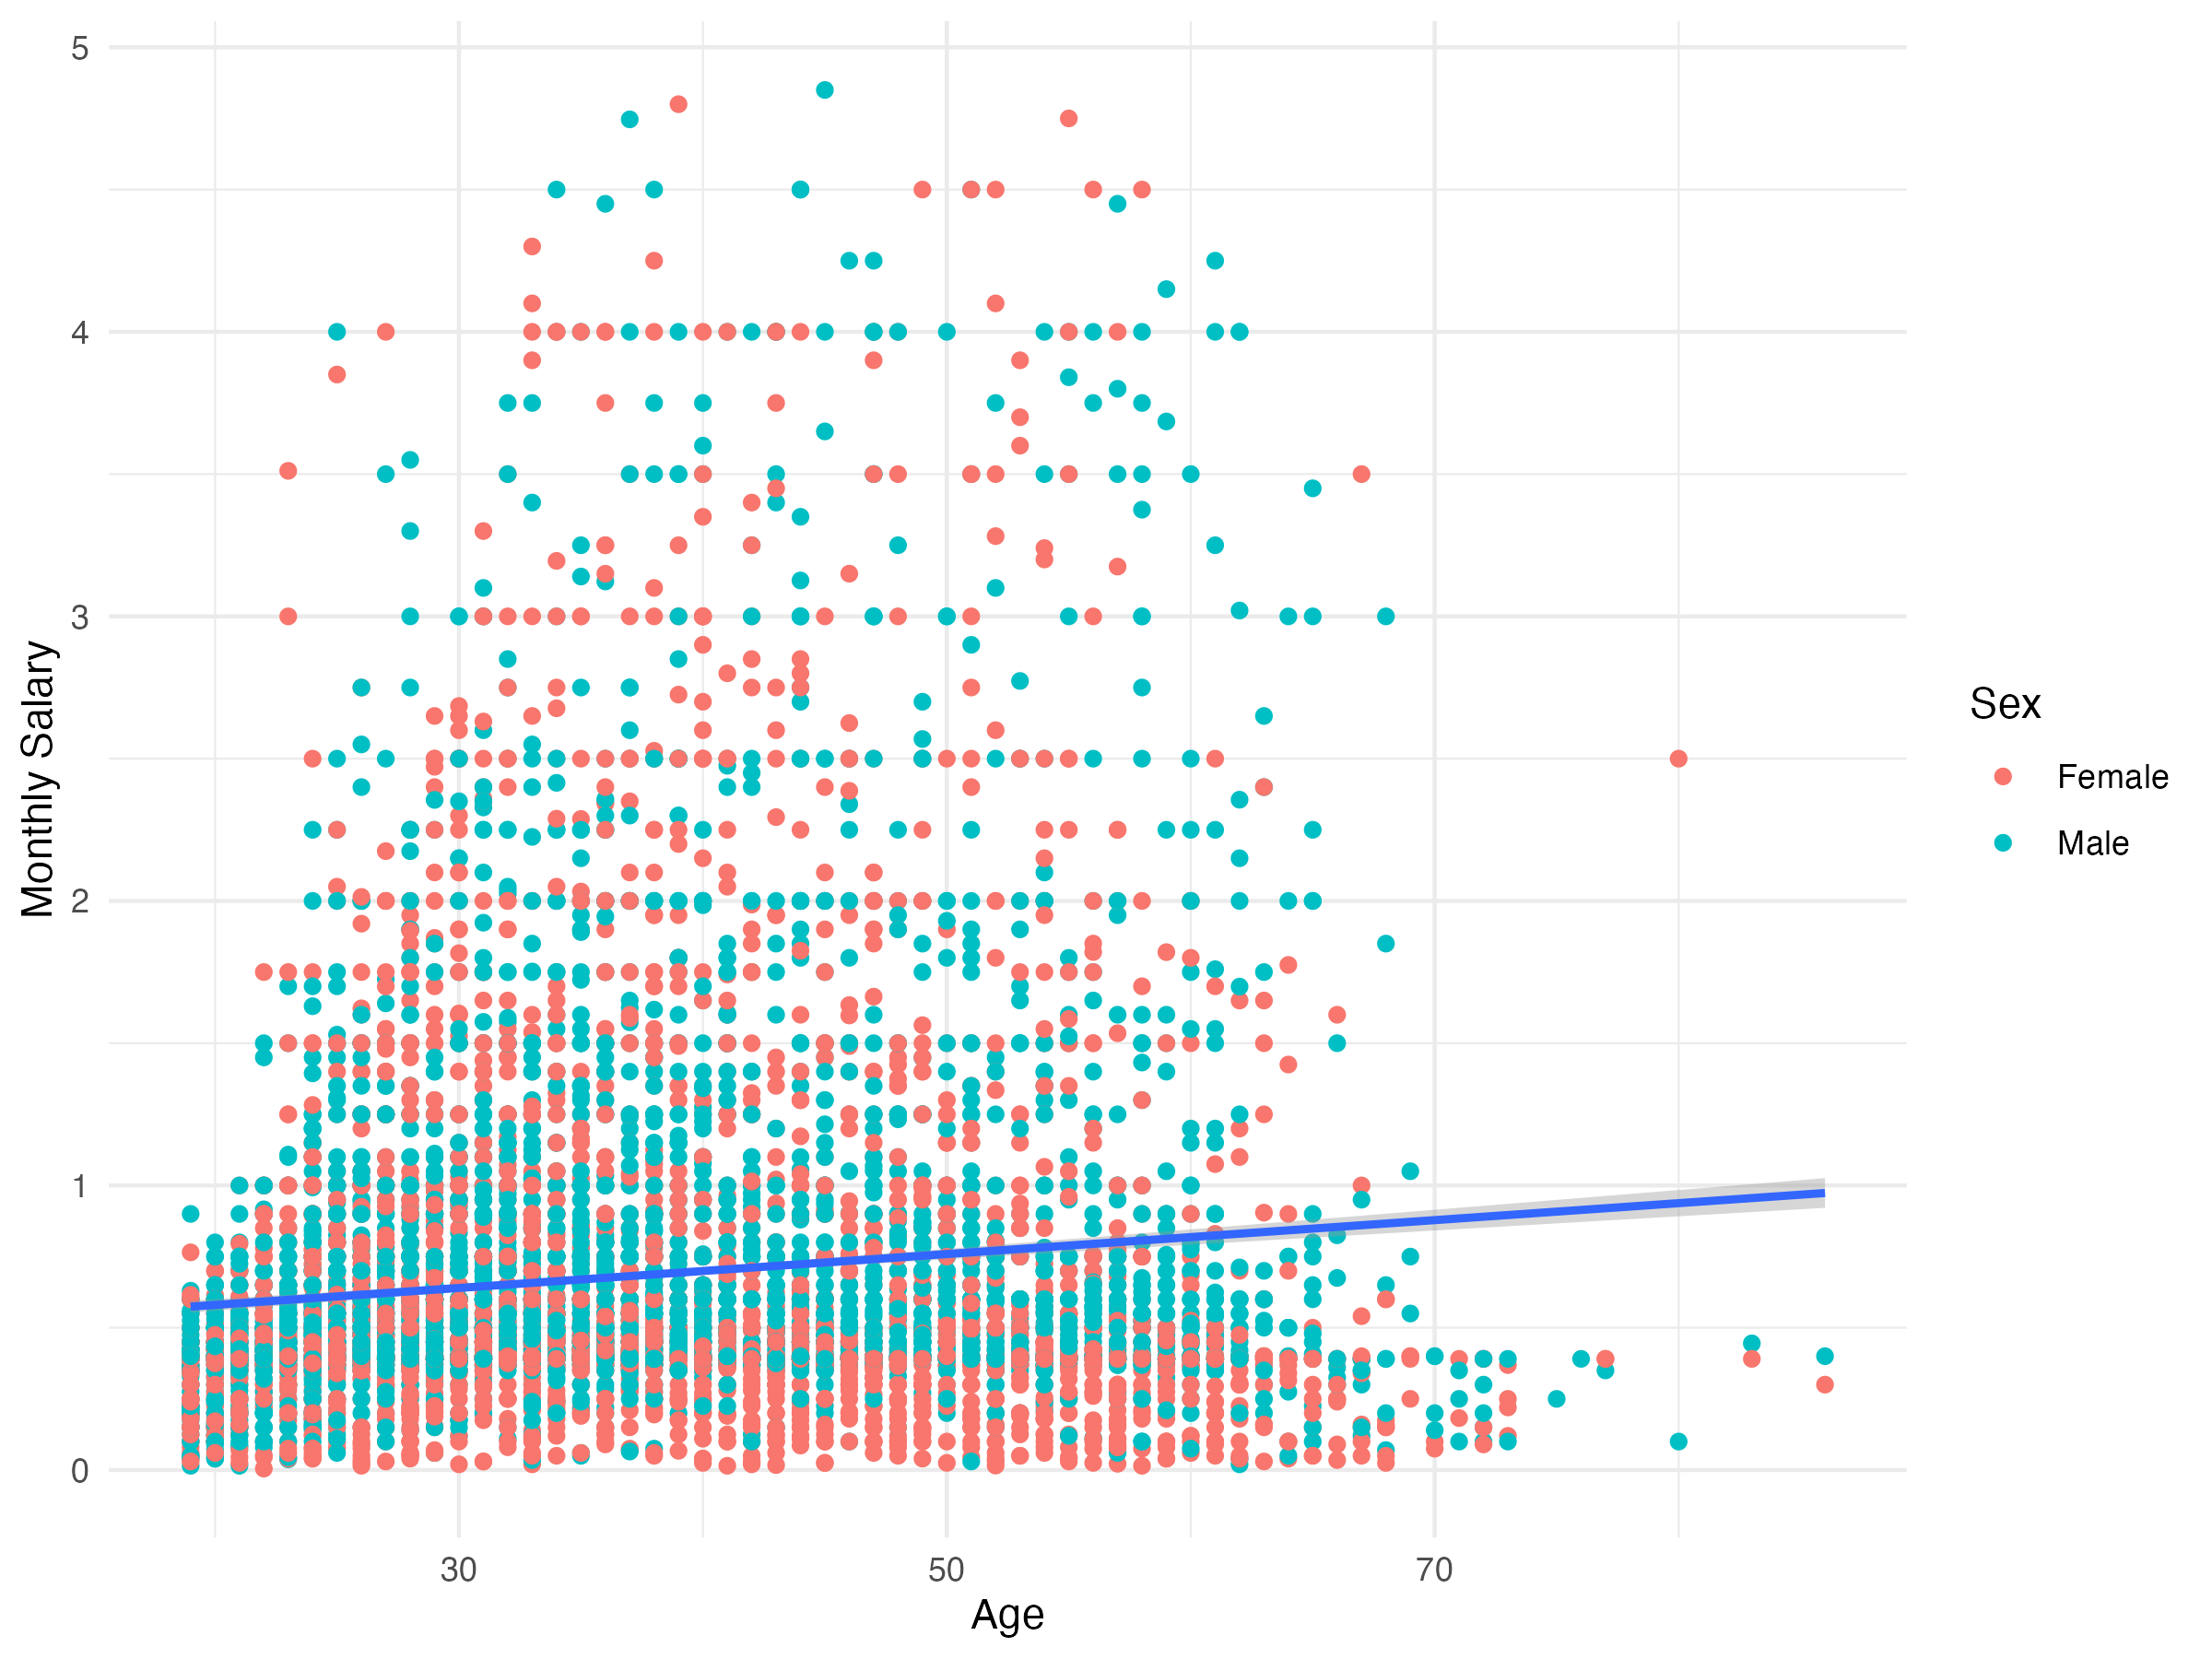
\includegraphics[scale=0.7]{../views/P01_salary_age_sex.png}   
        \caption{Monthly Salary--Age Distribution by Gender} \label{fig:P01}
    \end{figure}

     \textit{Figure 1} presents the relationship between monthly salary, age, and gender. The x-axis represents age, while the y-axis shows monthly salary (limited to 10 million COP for better visualization), with red dots representing males and green dots representing females. As shown by the trend line, wages tend to increase slightly with age, though this growth remains modest. The highest concentration of wages falls within the age range of 20 to 60 years, with significant dispersion in salaries as individuals grow older, especially after 50 years of age. This reflects the complex dynamics of salary distribution across different age groups in the labor market. Regarding the gender wage gap, although male and female salaries overlap in most ranges, the higher salary bracket (above 5 million COP) reveals a noticeable dominance of male workers. This pattern suggests a potential gender wage gap, particularly at higher income levels. Despite this, both men and women are subject to significant salary variation, which could be influenced by other key factors like education, job formality, or occupational roles beyond experience (age). The considerable variation in wages across ages underscores the intricate structure of the Bogota labor market, where educational attainment, job sector, and other characteristics may contribute to substantial differences in earnings across individuals.

    \begin{figure}[H]
        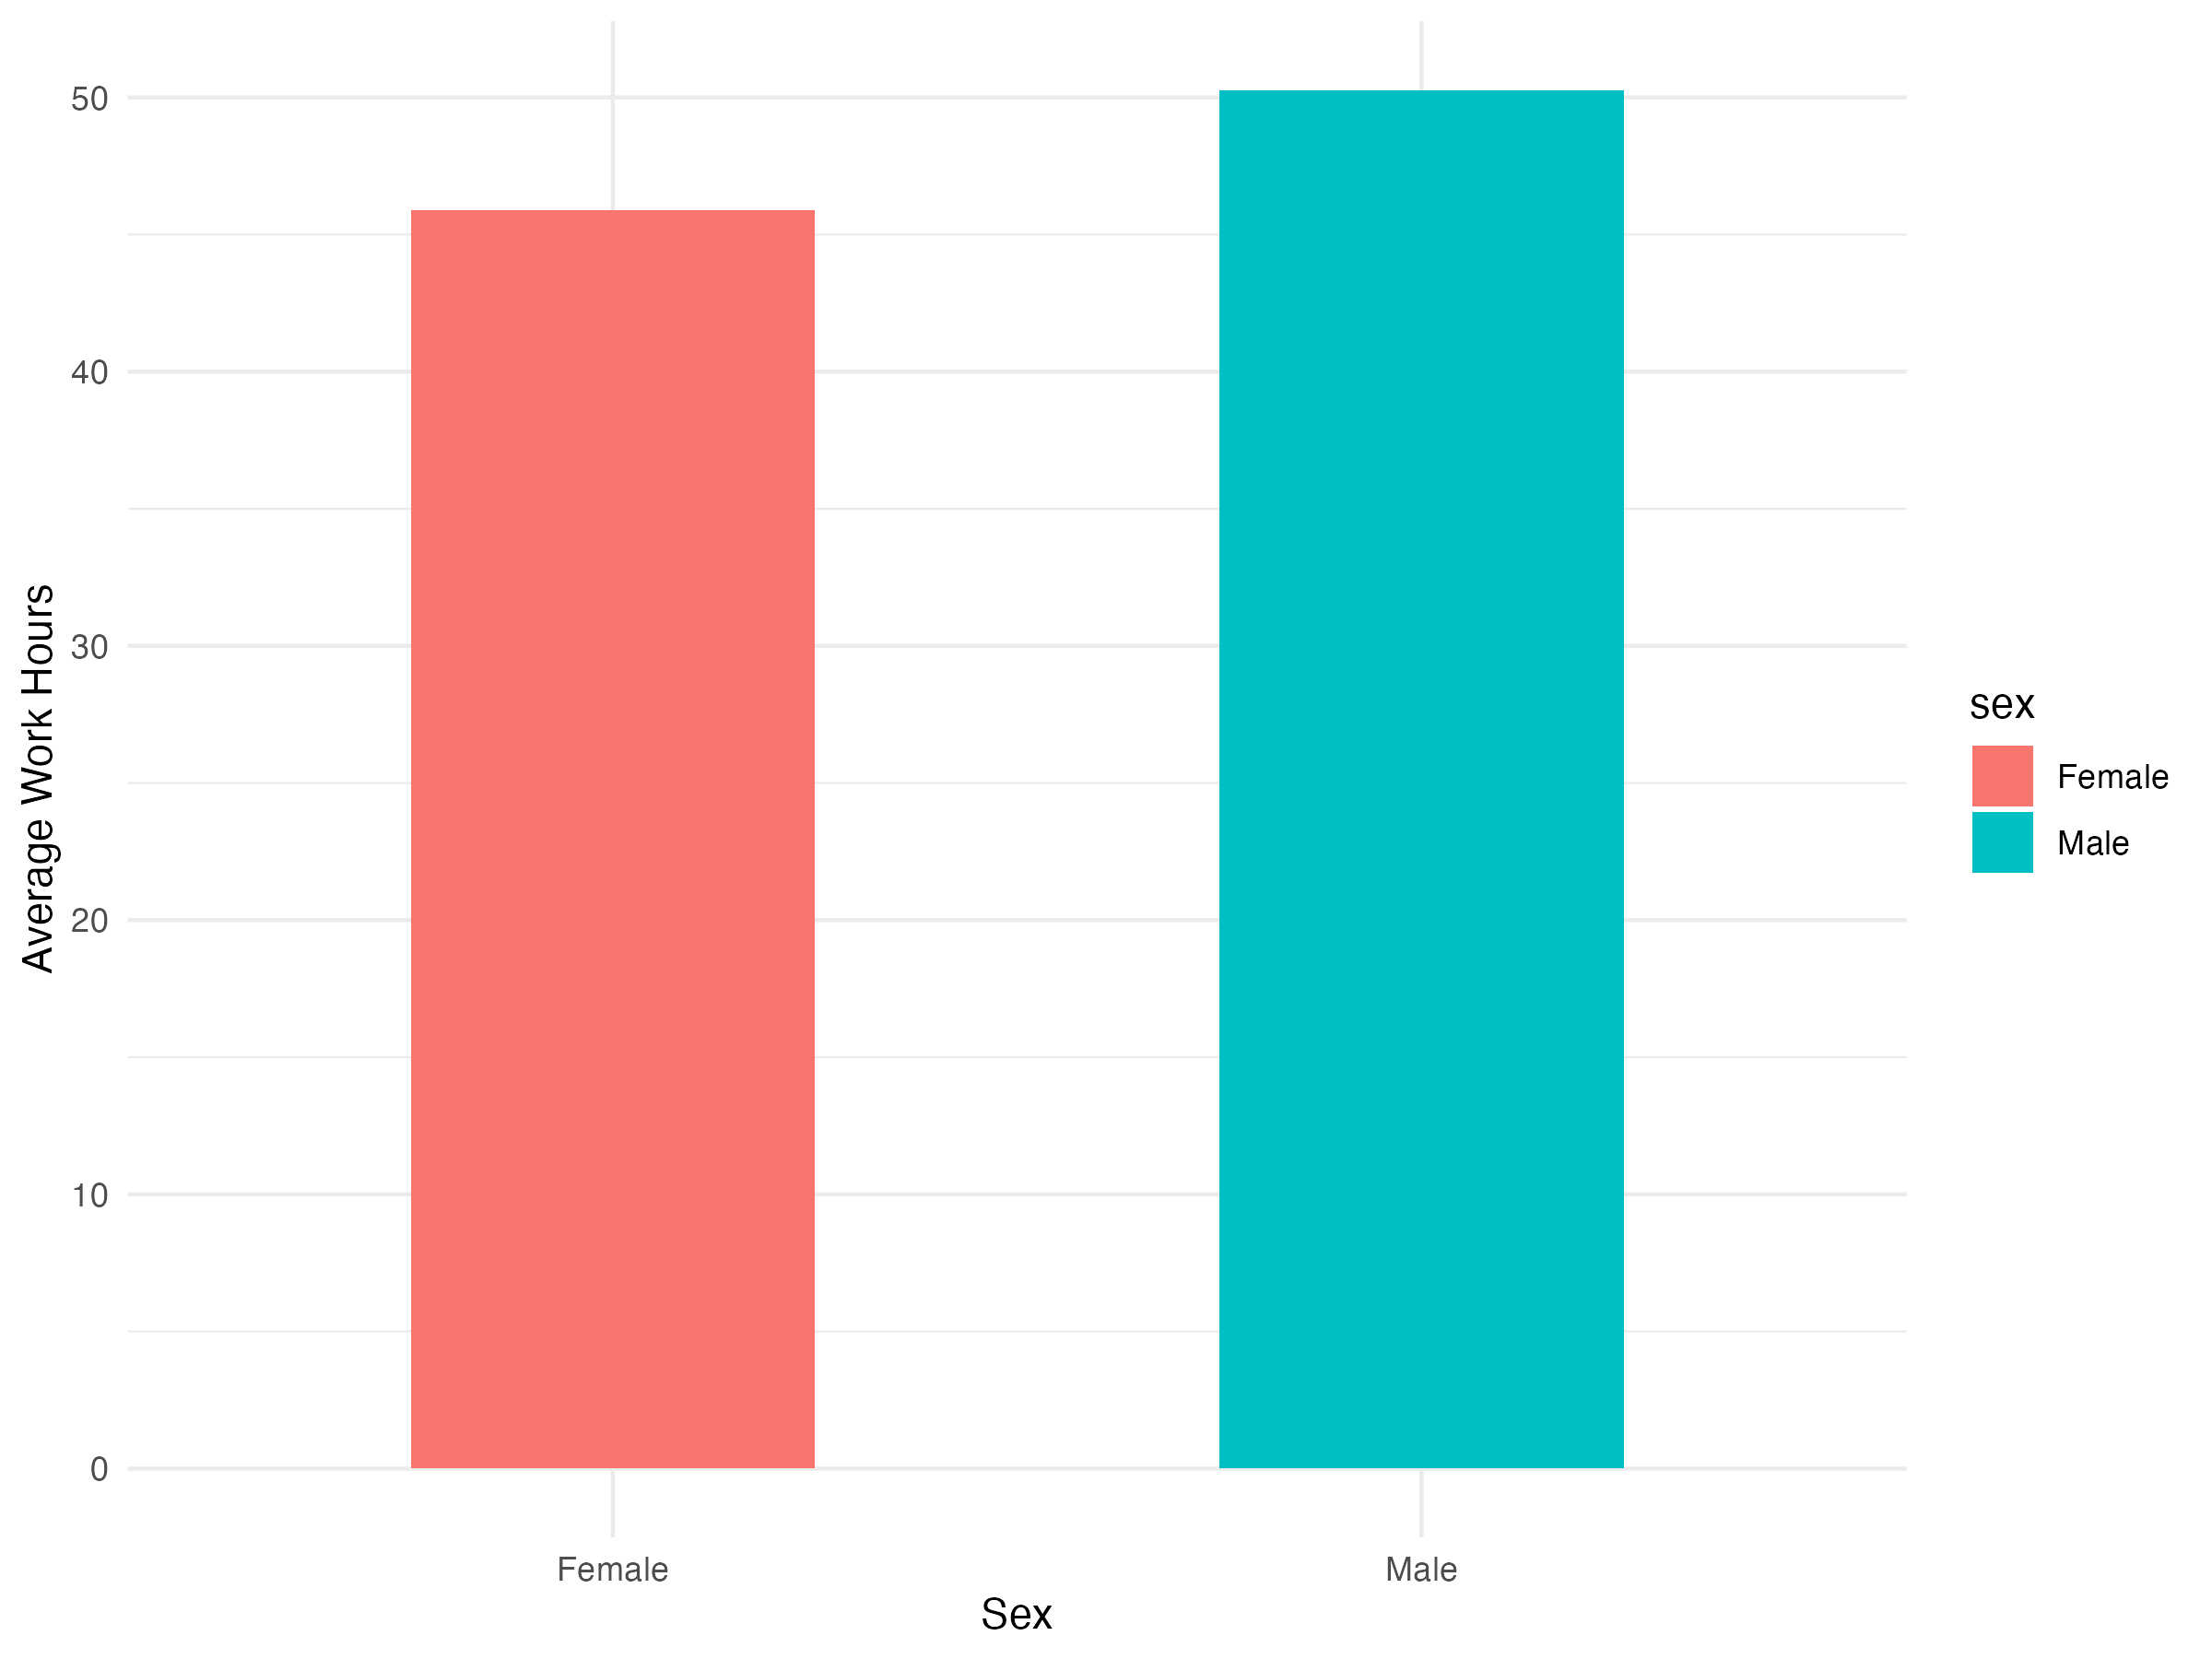
\includegraphics[scale=0.6]{../views/P02_work_hours_sex.png}   
        \caption{Comparison of Average Work Hours by Gender} \label{fig:P02}
    \end{figure}

    The bar chart in \textit{Figure 2} presents the comparison of average work hours between men and women. The x-axis classifies by gender, while the y-axis measures the average number of work hours per week. The data reveal that, on average, men work slightly more hours per week than women. Specifically, men register around 50 hours per week, while women work close to 45 hours. This 5-hour difference is notable and may have direct implications for the gender wage gap observed in the data. Several factors could explain this disparity. Women might be more likely to engage in part-time work or jobs that require fewer weekly hours, potentially due to sectors with reduced working hours. Additionally, domestic and caregiving responsibilities often fall disproportionately on women, limiting their availability for full-time work. This gap in work hours is important for understanding the gender wage gap, as working more hours is often correlated with higher earnings. Thus, analyzing both work hours and other relevant factors is essential when investigating wage differences across genders.

    \begin{figure}[H]
        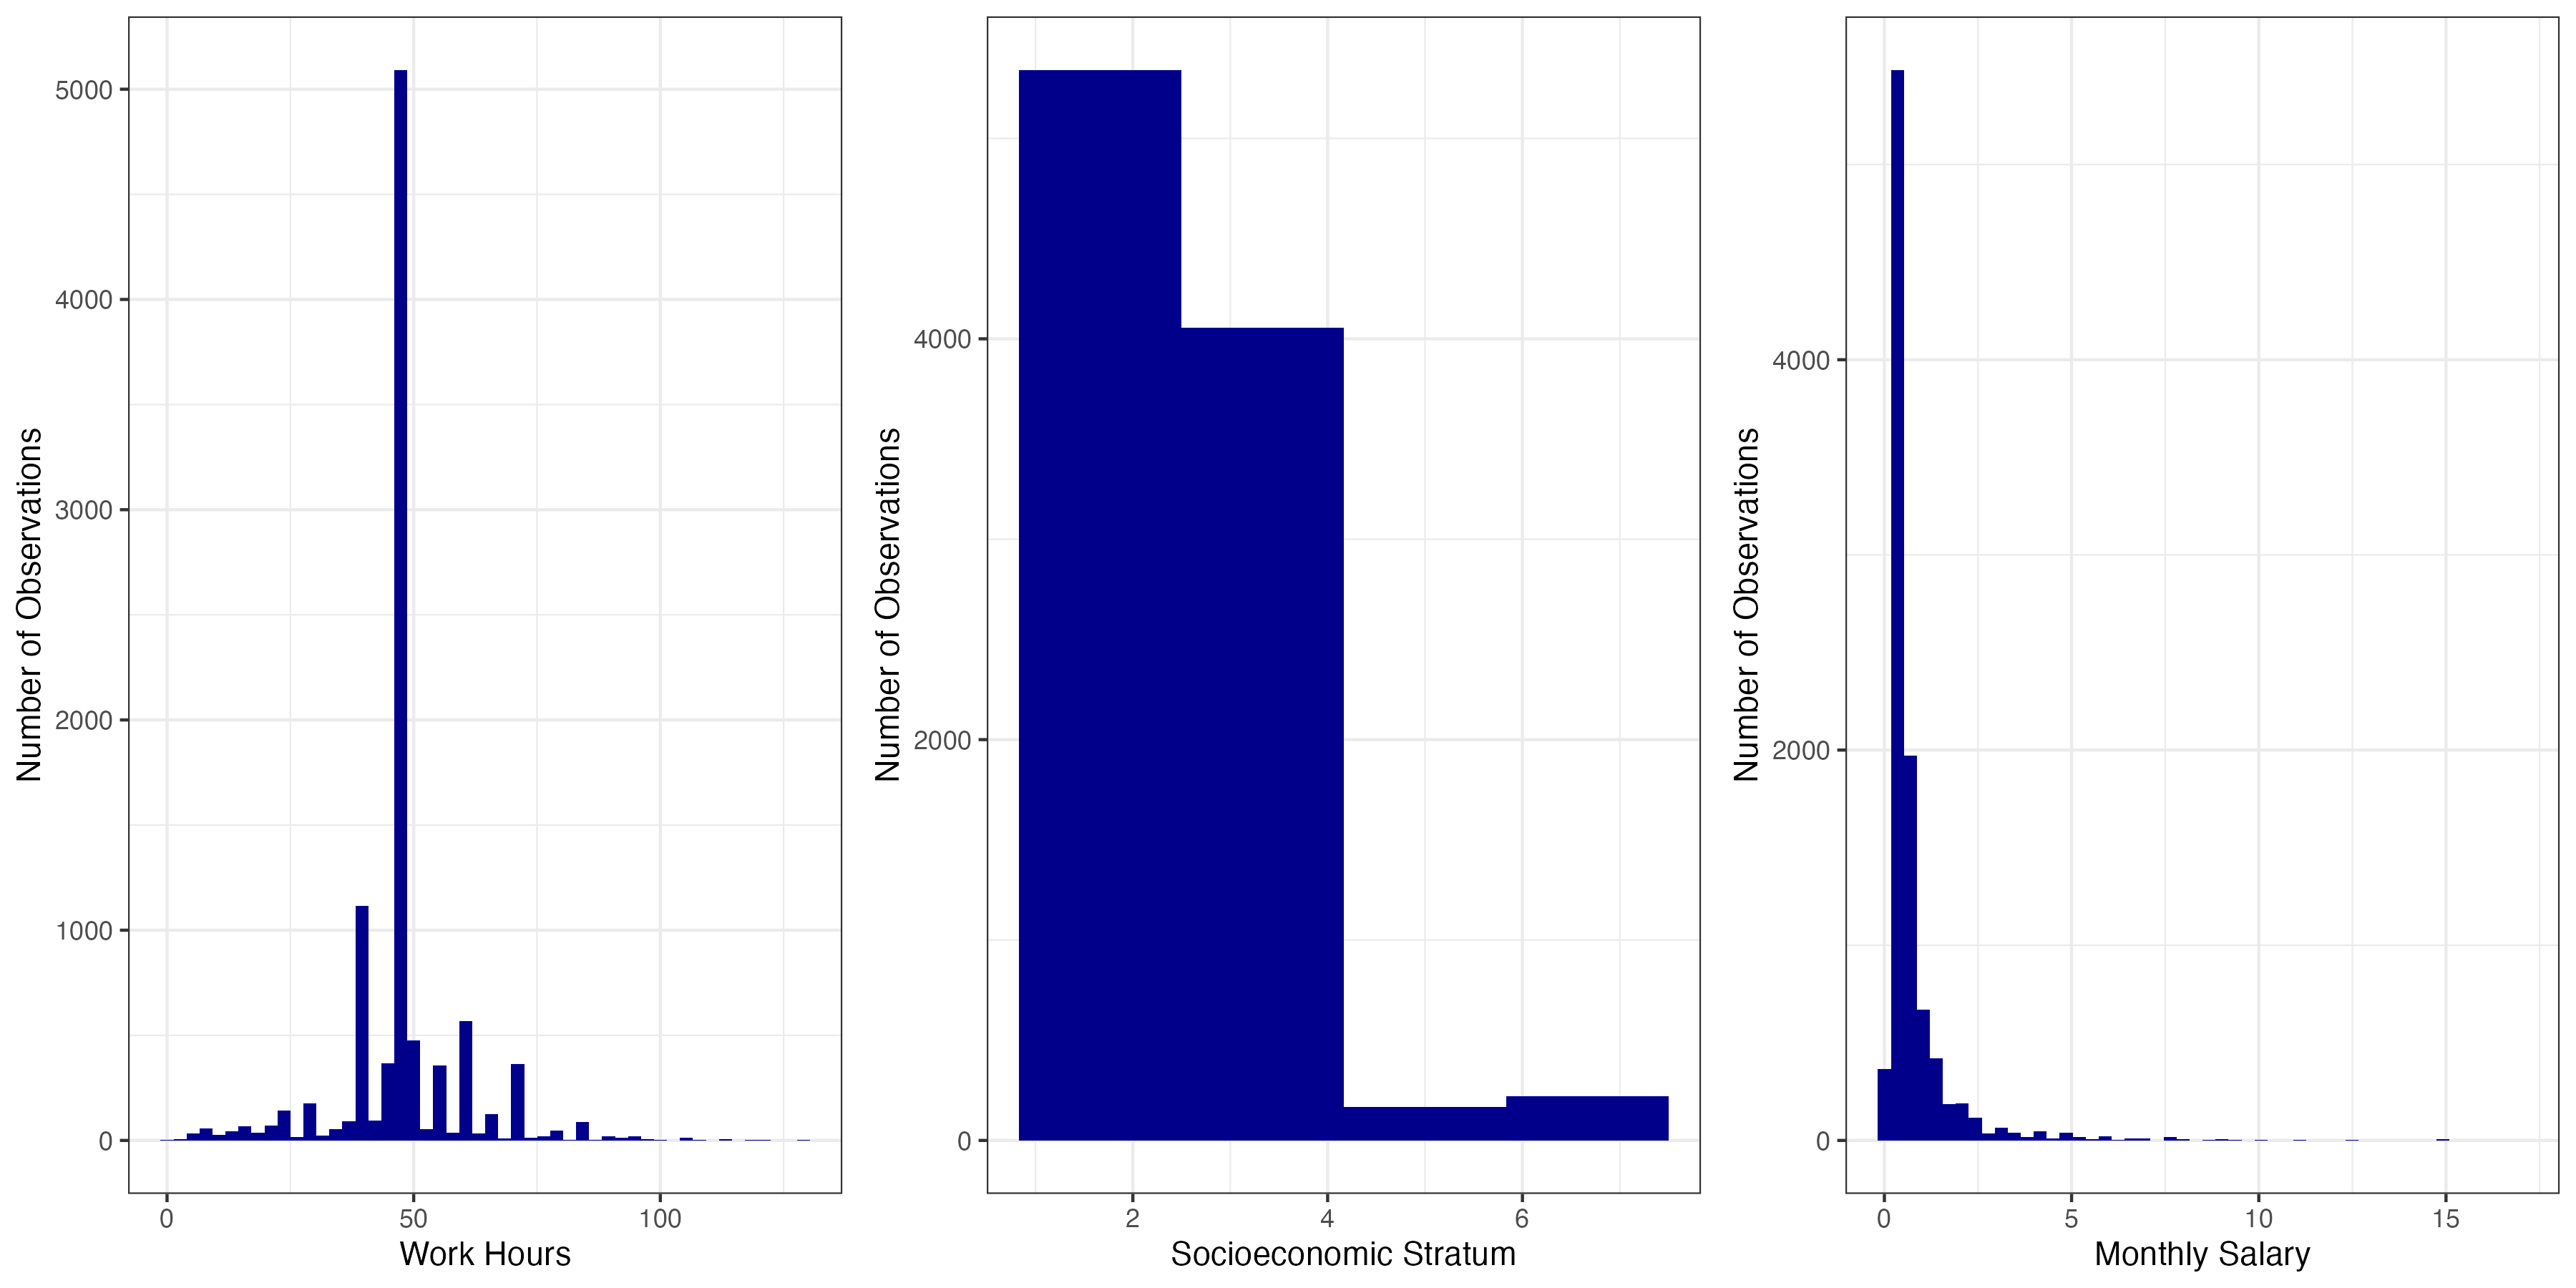
\includegraphics[scale=0.5]{../views/P03_histograms_combined.png}   
        \caption{Distribution of Work Hours, Socioeconomic Stratum, and Monthly Salary} \label{fig:P03}
    \end{figure}

    The distribution of work hours (left) in Figure 3 illustrates that the vast majority of workers are concentrated between 40 and 50 hours per week, with a noticeable peak around 48 hours. This is in line with the standard full-time work week in Colombia. However, the histogram also reveals a small but significant number of individuals working extreme hours, with some reporting over 100 hours per week. These extreme cases might reflect either overworked individuals or people holding multiple jobs. The variation in work hours is a key factor to consider in this analysis as it directly affects income levels and labor market participation, and it may be particularly relevant when exploring income disparities.
    
    The middle panel of Figure 3 shows the distribution of socioeconomic strata, where the majority of individuals fall within stratum 2 and stratum 3, representing the lower and lower-middle socioeconomic levels in Bogota. Very few individuals are from higher strata (5 and 6), which is expected given Bogota's socioeconomic composition. The heavy concentration in the lower strata highlights the prevalent inequality in the city and may explain significant variations in income, as individuals from lower strata likely face greater barriers to accessing high-paying jobs. Including this variable in the analysis is crucial for understanding how socioeconomic background influences wage outcomes.
    
    The right-hand side of Figure 3 displays the distribution of monthly salary, which is heavily skewed to the right. Most individuals earn less than 2 million COP per month, with a large concentration near the minimum wage. There is a small proportion of high-income earners, with some individuals making over 10 million COP, which significantly skews the data. This stark inequality in income distribution is indicative of broader structural disparities in Bogota's labor market, where only a minority benefit from high-wage opportunities while the majority earn relatively low wages. This underscores the importance of examining wage inequality and its determinants in the analysis.



% ---------------------------------------------------------------- %
% --------------------------- AGE-WAGE --------------------------- %
% ---------------------------------------------------------------- %

\section{Age-Wage Profile}

    A substantial body of evidence in labor economics suggests that the age-wage profile of a typical worker follows a predictable trajectory. Wages tend to be lower when a worker is young, rising as the worker ages, reaching a peak around age 50, and then stabilizing or slightly declining thereafter. In this section, we estimate the age-wage profile for the individuals in our sample using the following quadratic model:
    
    \begin{equation}
        \log(w) = \beta_1 + \beta_2 Age + \beta_3 {Age}^2 + u
    \end{equation}
    
    
% Table created by stargazer v.5.2.3 by Marek Hlavac, Social Policy Institute. E-mail: marek.hlavac at gmail.com
% Date and time: Sun, Sep 15, 2024 - 10:40:12
\begin{table}[!htbp] \centering 
  \caption{Regression Results: Log Wage as a Function of Age} 
  \label{} 
\begin{tabular}{@{\extracolsep{5pt}}lc} 
\\[-1.8ex]\hline 
\hline \\[-1.8ex] 
 & \multicolumn{1}{c}{\textit{Dependent variable:}} \\ 
\cline{2-2} 
\\[-1.8ex] & Log Wage \\ 
\hline \\[-1.8ex] 
 Age & 0.079$^{***}$ \\ 
  & (0.004) \\ 
  & \\ 
 Age2 & $-$0.001$^{***}$ \\ 
  & (0.00005) \\ 
  & \\ 
 Constant & 12.380$^{***}$ \\ 
  & (0.073) \\ 
  & \\ 
\hline \\[-1.8ex] 
Peak Age & 43.3 \\ 
95% CI for Peak Age (Bootstrap) & 42.42 - 44.39 \\ 
Observations & 9,784 \\ 
R$^{2}$ & 0.045 \\ 
\hline 
\hline \\[-1.8ex] 
\textit{Note:}  & \multicolumn{1}{r}{$^{*}$p$<$0.1; $^{**}$p$<$0.05; $^{***}$p$<$0.01} \\ 
\end{tabular} 
\end{table} 
%
    
    The results of the regression can be seen in \textit{Table 2}. The coefficient on the linear term for age is 0.079 and is statistically significant at the 1\% level. This indicates that for every additional year of age, there is an approximate 7.9\% increase in the wage rate, holding everything else constant. However, the quadratic term for age is negative (-0.001) and also highly significant, suggesting that the effect of age on wages diminishes as workers grow older. The negative coefficient on the squared term ($\beta_3 = -0.001$) captures the concave relationship between age and wages. Specifically, while wages initially rise with age, the positive effect diminishes as workers get older, eventually leading to a decline in wages. This is consistent with the standard age-wage profile in labor economics, where wages peak at a certain age and then taper off. From the estimates, we calculate the peak wage occurs at approximately 43.3 years of age, based on the formula for the critical point of a quadratic function. The 95\% confidence interval for this peak age, computed using bootstrap methods, ranges from 42.42 to 44.39 years, indicating that the peak is relatively well-defined and not overly sensitive to sampling variability.
    
    
    The model's $R^2$ is 0.045, meaning that only about 4.5\% of the variance in log wages is explained by age and age squared. This relatively low $R^2$ suggests that while age plays a role in determining wages, it is far from the sole determinant. Other unobserved factors, such as education, experience, and occupation, likely explain a significant portion of wage variation. However, the significance of both the age and age-squared coefficients implies that age alone does have a meaningful, although not overwhelming, impact on wages. The concavity of the age-wage profile reflects that while wages increase during early and mid-career stages, they do eventually decline as workers approach the later stages of their working lives. This pattern is consistent with human capital theory, where initial investments in skills and experience yield returns, but those returns diminish with time as the depreciation of skills and physical capacity take hold. Overall, this model captures the broad contours of the age-wage relationship, confirming that wages peak around middle age and decline thereafter. However, the low $R^2$ suggests that further exploration with additional covariates may improve the explanatory power of the model.

    \begin{figure}[H]
        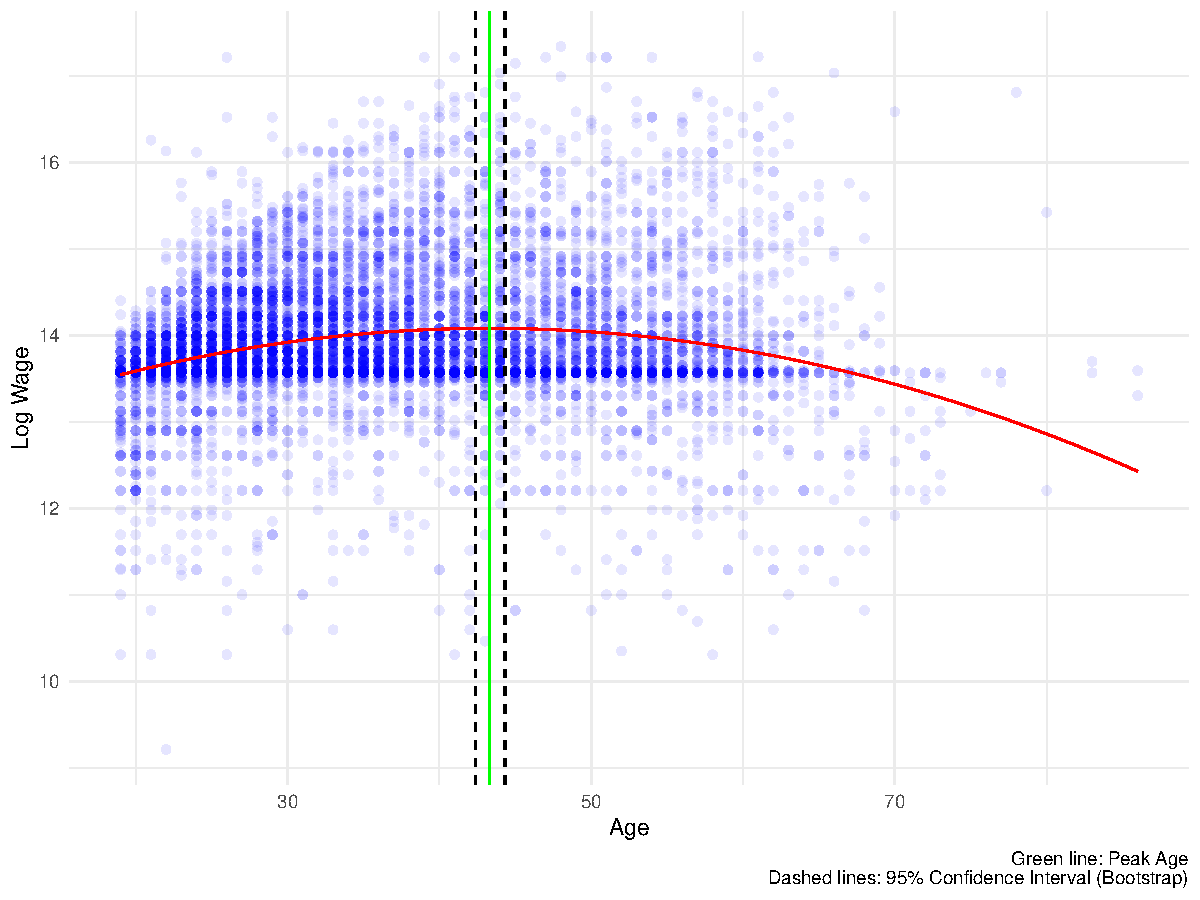
\includegraphics[scale=0.6]{../views/P1_age_log_wage_profile.pdf}   
        \caption{Age--LogWage Profile} \label{fig:P1}
    \end{figure}
    
    \begin{figure}[H]
        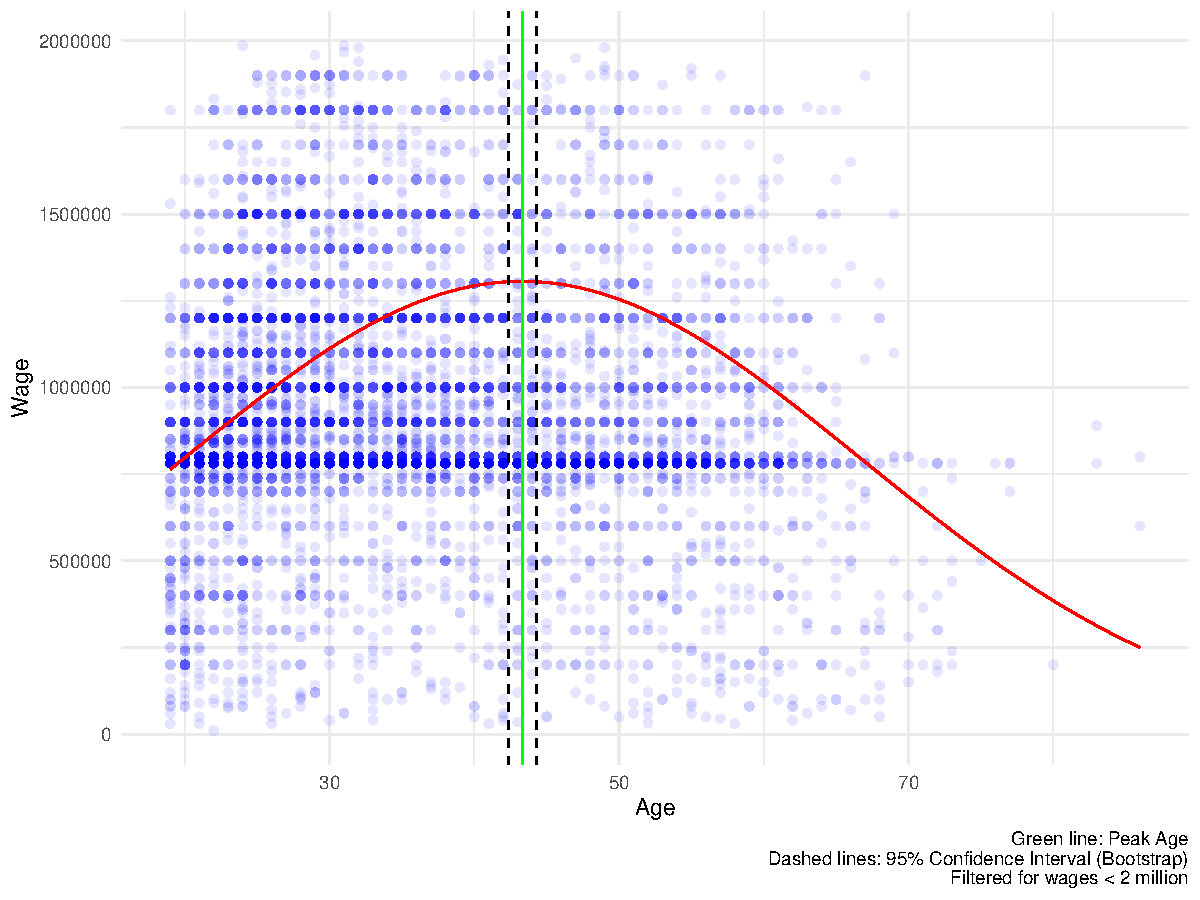
\includegraphics[scale=0.6]{../views/P2_age_wage_profile.pdf}   
        \caption{Age--Wage Profile } \label{fig:P2}
    \end{figure}
    
    \begin{figure}[H]
        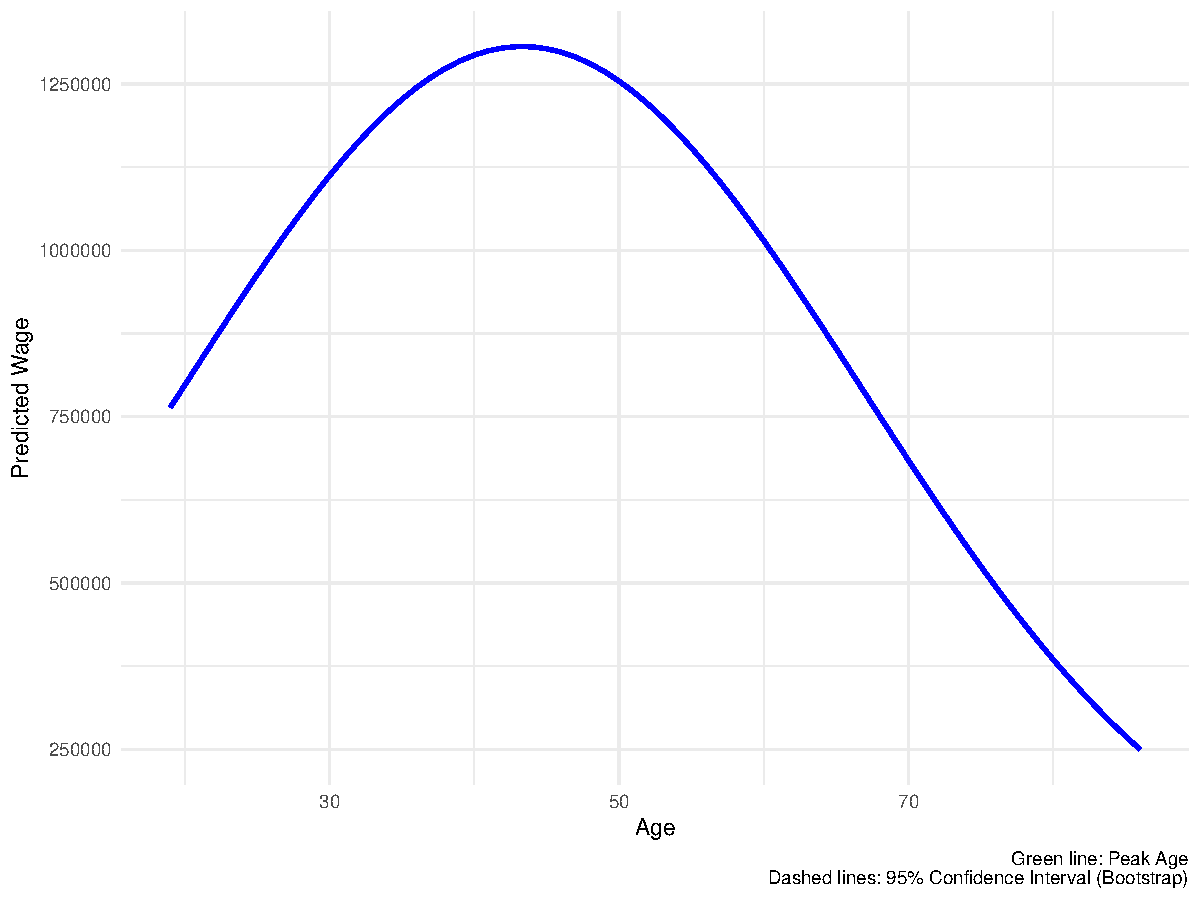
\includegraphics[scale=0.6]{../views/P3_age_wage_profile2.pdf}   
        \caption{Predicted Age--Wage } \label{fig:P3}
    \end{figure}

    In the first plot (\textit{Figure 1}), we can observe the relationship between age and log wages, fitted with the quadratic model. The scatter plot shows the log wages of individuals at different ages, with the red curve representing the predicted values from the regression model. The green vertical line marks the estimated peak age at around 43.3 years, with the dashed black lines representing the 95\% confidence interval for the peak age, ranging from approximately 42.42 to 44.39 years. The model captures the concave shape of the age-wage profile, where wages increase with age until the peak, after which they start to decline. However, this decline is quite sharp, which may not entirely align with what is generally observed in the labor economics literature, where wages tend to stabilize after reaching the peak rather than falling dramatically. The steep decline after the peak suggests that the quadratic model may oversimplify the relationship, as it does not account for additional factors that could influence wage stability, such as seniority, promotions, or experience accumulation that could maintain wages even after the age of 50.

    In \textit{Figure 2}, the focus shifts from log wages to actual wages, making it easier to visualize the monetary wage distribution across ages. To make the pattern more discernible, wages greater than 2 million have been filtered out. This allows us to better see the overall wage distribution and its quadratic fit, avoiding the distortion that extreme outliers could introduce. The pattern remains consistent with \textit{Figure 1}. The red curve follows a similar trajectory, but the filtered wage data highlights the wage pattern for the majority of the workers in this sample. The exclusion of high wage outliers allows us to observe the general trend more clearly. Nevertheless, as in \textit{Figure 1}, the decline after the peak is sharper than expected according to economic theories, which typically predict a plateau or slight decline in wages rather than a sharp drop after a certain age.
    
    \textit{Figure 3} plots the predicted wages by age, showing the quadratic fit. Here, we see that the predicted wage peaks at around 1.25 million before dropping again. This decline is again exaggerated due to the simplicity of the quadratic model, and it fails to capture the wage stability expected after the peak in older ages. The focus on age alone, without considering other relevant factors, such as education, experience, industry, or sex, could explain why the model predicts such a sharp drop. A more robust model that includes these factors might predict a more gradual decline or even a plateau post-peak, in line with empirical evidence from labor economics. 



% ---------------------------------------------------------------- %
% -------------------------- GENDER GAP -------------------------- %
% ---------------------------------------------------------------- %

\section{The Gender Earnings GAP}

    \subsection{Unconditional Gap}

        Policymakers have long been concerned with the gender wage gap, and it is the focus of this subsection. The gender wage gap can be quantified by estimating a simple regression where the log wage is regressed on an indicator variable for gender. Specifically, we estimate the following model:
    
        \begin{equation}
            log(w) = \beta_1 + \beta_2 Female + u
        \end{equation}
        
        In this model, the variable \textit{Female} is an indicator variable that takes the value 1 if the individual is identified as female and 0 otherwise. The coefficient $\beta_2$ provides an estimate of the unconditional wage gap between males and females, with a negative value indicating that females earn less than males on average.
        
        
% Table created by stargazer v.5.2.3 by Marek Hlavac, Social Policy Institute. E-mail: marek.hlavac at gmail.com
% Date and time: Sun, Sep 15, 2024 - 10:40:19
\begin{table}[!htbp] \centering 
  \caption{Gender Wage Gap: Simple, Conditional, and FWL Models} 
  \label{} 
\begin{tabular}{@{\extracolsep{5pt}}lccc} 
\\[-1.8ex]\hline 
\hline \\[-1.8ex] 
 & \multicolumn{3}{c}{\textit{Dependent variable:}} \\ 
\cline{2-4} 
\\[-1.8ex] & \multicolumn{2}{c}{Log Wage} & resid\_lw\_controls \\ 
\\[-1.8ex] & (1) & (2) & (3)\\ 
\hline \\[-1.8ex] 
 Female & $-$0.153$^{***}$ & $-$0.069$^{***}$ &  \\ 
  & (0.015) & (0.014) &  \\ 
  & & & \\ 
 resid\_female\_controls &  &  & $-$0.069$^{***}$ \\ 
  &  &  & (0.000) \\ 
  & & & \\ 
 Constant & 13.987$^{***}$ & 12.296$^{***}$ & 0.000 \\ 
  & (0.011) & (0.044) & (0.014) \\ 
  & & & \\ 
\hline \\[-1.8ex] 
Observations & 9,784 & 9,784 & 9,784 \\ 
R$^{2}$ & 0.010 & 0.258 & 0.003 \\ 
\hline 
\hline \\[-1.8ex] 
\textit{Note:}  & \multicolumn{3}{r}{$^{*}$p$<$0.1; $^{**}$p$<$0.05; $^{***}$p$<$0.01} \\ 
\end{tabular} 
\end{table} 
%
        
        The results of the regression are presented in \textit{Table 3}. The coefficient on the \textit{Female} variable is -0.153, and it is statistically significant at the 1\% level. This suggests that, on average, women in the sample earn approximately 15.3\% less than men, all else being equal. The constant term of 13.987 represents the average log wage for males in the sample. The $R^2$ value of the model is 0.01, which means that gender alone explains only about 1\% of the variation in log wages. This is not surprising, as wages are determined by a variety of factors beyond gender, such as education, experience, occupation, and industry. However, the fact that the gender coefficient is significant and negative indicates the presence of an unconditional wage gap between men and women.
        
        This model captures the broad difference in earnings between genders, but it does not account for any other factors that might explain the gap, such as differences in education levels, work experience, or job types between men and women. These factors could potentially explain part of the observed wage disparity, meaning that this unconditional gap likely overstates the true gender wage gap that could exist once these variables are taken into account. This simple regression highlights the existence of a gender earnings gap in the sample, with women earning significantly less than men on average. However, a more detailed model that controls for additional variables would be necessary to understand the full extent and causes of the gender wage gap.
            


    \subsection{Equal Pay for Equal Work}
        
        A common slogan in discussions of labor market inequality is "equal pay for equal work," which suggests that for employees with similar worker and job characteristics, no gender wage gap should exist. To investigate this claim, we estimate the conditional gender wage gap, controlling for factors that reflect similar job and worker characteristics. In particular, we incorporate control variables that capture differences in the type of work, working hours, formality of employment, and the size of the firm. These factors are important as they influence wages and can help isolate the true impact of gender on earnings. The model we estimate is:
        \begin{equation}
            log(w) = \beta_1 + \beta_2 {Female} + \beta_3 {Relab} + \beta_4 {Hours Worked} + \beta_5 {Formality} + \beta_6 {FirmSize} + u
        \end{equation}
        
        In this specification, we control for the variable \textit{relab}, which indicates the type of job relationship (e.g., employee, self-employed), \textit{hoursWorkUsual}, which captures the usual number of hours worked per week, \textit{formal}, an indicator of whether the individual works in the formal sector, and \textit{sizeFirm}, representing the size of the firm. These variables reflect important job characteristics that can impact wages, allowing us to estimate a "conditional" wage gap that accounts for differences in job and worker traits. We estimate the conditional gender wage gap using the Frisch-Waugh-Lovell (FWL) theorem, which allows us to partial out the effects of the control variables before estimating the effect of gender on wages. The two steps of FWL are as follows:
        \begin{equation}
            Resid_{Female} = \beta_1 + \beta_2 {Relab} + \beta_3 {Hours Worked} + \beta_4 {Formality} + \beta_5 {FirmSize} + u
        \end{equation}
        \begin{equation}
            Resid_{log(w)} = \beta_1 + \beta_2 {Relab} + \beta_3 {Hours Worked} + \beta_4 {Formality} + \beta_5 {FirmSize} + u
        \end{equation}


        The regression of the residuals of \textit{log(wage)} on the residuals of \textit{Female} gives us the conditional gender wage gap, after controlling for job and worker characteristics. The results are presented in \textit{Table 3}. In \textit{Table 4}, we report both the standard errors from the FWL estimation and the standard errors obtained via bootstrap with 1,000 replications to assess the robustness of the estimates.
        
        
\begin{table}[ht]
\centering
\begin{tabular}{l c}
\hline
 & Statistic \\
\hline
Coefficient &  -0.06873  \\
Standard Error &  0.01354  \\
Standard Error (Bootstrap) &  0 0.01376  \\
\hline
\end{tabular}
\caption{FWL Coefficient and Standard Errors Comparison}
\label{tab:fwl_comparison}
\end{table}
%
        
        The estimated gender wage gap models, presented in \textit{Table 3}, provide a comprehensive analysis of the unconditional and conditional differences in wages between men and women. The first model estimates the unconditional wage gap using a simple regression where log wages are regressed solely on the \textit{Female} indicator. The second and third models introduce controls for job and worker characteristics using a more detailed specification and the Frisch-Waugh-Lovell (FWL) theorem, respectively. The objective of this section is to interpret the economic and statistical significance of the results, as well as to reflect on whether the observed differences are due to selection bias, discrimination, or other factors. The first model (unconditional) regresses log wages on the \textit{Female} variable alone, revealing a significant gender wage gap of approximately 15.3\%. This suggests that women earn, on average, 15.3\% less than men in the sample. However, this model is limited because it does not account for the fact that men and women might differ in terms of job characteristics, such as occupation type, working hours, or formality of employment. Thus, while the unconditional wage gap is economically significant, it cannot provide a complete understanding of the underlying causes of the wage disparity.
        
        The second model includes control variables to account for differences in employment type (\textit{relab}), hours worked per week (\textit{hoursWorkUsual}), formality (\textit{formal}), and firm size (\textit{sizeFirm}). Each of these controls is crucial in explaining wages. Employment type (\textit{relab}) is important because self-employed workers or independent contractors often earn differently than employees, while working hours can directly affect income. Formality is critical in distinguishing between workers with access to social benefits and job protections versus those in more precarious, informal work. Finally, firm size tends to correlate with wage levels, as larger firms often offer higher salaries due to greater resources and more competitive compensation structures. With the inclusion of these controls, the wage gap narrows to 6.9\%, a substantial reduction from the unconditional gap. This indicates that a significant portion of the wage difference between men and women can be attributed to differences in job characteristics. The controls explain much of the wage variation, which is reflected in the $R^2$ value, which increases to 0.258. This suggests that about 25.8\% of the variation in wages is explained by the included job and worker characteristics, a notable improvement from the 1\% explained by gender alone in the first model.
        
        The third model applies the Frisch-Waugh-Lovell (FWL) theorem, which partials out the effects of the control variables before estimating the effect of gender on wages. The estimated coefficient for \textit{Female} remains -0.069, the same as in the second model. This confirms that the conditional wage gap does not change when using FWL, and the residuals are estimated efficiently. The interpretation of this gap remains the same: women earn approximately 6.9\% less than men after accounting for job characteristics. The robustness of this estimate is confirmed by the comparison of standard errors presented in \textit{Table 4}. The standard error from the FWL model is 0.01354, while the bootstrapped standard error is nearly identical at 0.01376. This suggests that the FWL estimate is robust and reliable, as the inclusion of the bootstrapped standard error confirms the precision of the model's estimate.
        
        With that in mind, the significant reduction in the gender wage gap from 15.3\% in the unconditional model to 6.9\% in the conditional models suggests that much of the observed wage difference is driven by differences in job characteristics between men and women. These characteristics include employment type, working hours, formality, and firm size, all of which are known to affect wages. However, the fact that a wage gap of 6.9\% remains even after controlling for these factors raises important questions. This residual wage gap may reflect a combination of factors, including selection bias and discrimination. Selection bias could arise if women systematically select, or are selected into, lower-paying jobs, either due to preferences or constraints (e.g., family responsibilities, labor market structures). However, even after accounting for these observable job characteristics, the persistence of a gender wage gap suggests that discrimination—either explicit or implicit—could also be playing a role. Discriminatory practices in hiring, promotion, and pay-setting, as well as differences in negotiation or access to high-paying jobs, may contribute to the observed gap. Therefore, the reduction in the wage gap from the unconditional to the conditional models indicates that some of the gap is due to differences in job characteristics. However, the remaining conditional wage gap likely reflects a combination of unobserved factors, including potential discrimination or other barriers faced by women in the labor market. Further investigation, perhaps with additional controls for experience, education, and occupation, could help disentangle the relative contributions of these different factors to the gender wage gap.
    

        
\begin{table}[ht]
\centering
\begin{tabular}{lccc}
\hline
Sex & Peak Age & 95\% CI Lower & 95\% CI Upper \\
\hline
Male &  46.47  &  45.02  &  48.43  \\
Female &  40.39  &  39.46  &  41.53  \\
\hline
\end{tabular}
\caption{Peak Age and 95\% Bootstrap Confidence Intervals by Sex}
\label{tab:peak_age}
\end{table}
%

        The results in \textit{Table 5} highlight the estimated peak ages for men and women, along with their corresponding 95\% confidence intervals. According to the estimates, men reach their peak wage at 46.47 years of age, while women reach their peak earlier, at 40.39 years. The confidence interval for men ranges from 44.97 to 48.39, while for women it is narrower, ranging from 39.46 to 41.53. The difference in peak ages is notable, as the confidence intervals for men and women do not overlap, indicating that these peak ages are statistically different. This finding suggests that men experience a longer period of wage growth, potentially due to uninterrupted career paths and steady job progression. In contrast, women’s earlier peak age may reflect structural barriers or life events, such as caregiving responsibilities, that impact their long-term earnings potential.
        
        The disparity in peak ages also suggests that gender wage inequality may not be solely explained by differences in job characteristics or experience. Instead, these results point to more complex dynamics at play. For women, the earlier wage peak and subsequent decline could indicate that they face more significant challenges in maintaining high earnings as they age. This could be related to factors such as career interruptions, glass ceilings, or discrimination in promotions and wage increases. For men, the later peak and more gradual decline may reflect the accumulation of experience and seniority over time, as well as greater access to high-paying jobs later in life. The statistical difference between the peak ages further supports the conclusion that the labor market treats men and women differently, and that gender wage gaps are not purely the result of differences in job or worker characteristics.
        
        Moving on to the graphical analysis, \textit{Figure 4} shows the predicted age-wage profiles for both genders, with log wages plotted against age. The concave shape of the curve is consistent with the theoretical expectation that wages rise with age until they reach a peak, after which they decline. The vertical lines represent the estimated peak ages for men and women, with dashed lines marking the confidence intervals. The earlier peak for women is visually apparent, and the tighter confidence intervals around women’s peak age indicate less variation in the age at which women reach their wage maximum. The sharper decline in wages for women post-peak may suggest that women are more likely to experience wage stagnation or reductions as they age, possibly due to fewer opportunities for advancement or the impact of career breaks. For men, the wage growth continues for a longer period, and the post-peak decline is more gradual, indicating a more stable wage trajectory over time.
        
        In \textit{Figure 5}, which focuses on actual wages (capping them at 2 million COP to avoid distortions from extreme values), the patterns observed in \textit{Figure 4} are reinforced. The quadratic model continues to show a pronounced difference between men and women in terms of peak wage age and the rate of wage decline after the peak. The exclusion of outliers allows for a clearer view of the wage patterns for most of the sample. Once again, the earlier wage peak for women suggests that they face barriers that limit their wage growth compared to men. The steep decline in wages after the peak, particularly for women, underscores the fact that simply being of working age does not guarantee steady wage growth, as structural and individual-level factors can cause wage stagnation or even regression.
        
        Finally, in \textit{Figure 6}, the predicted wages for men and women based on the quadratic model provide further evidence of the gender wage gap over the life course. Men's predicted wages are consistently higher than women's, and their wage peak occurs later in life. For women, wages rise more slowly, peak earlier, and then decline at a sharper rate. This suggests that while both genders experience a rise and fall in wages over time, the trajectory is more favorable for men. The persistence of this wage gap, even after controlling for factors such as job characteristics and hours worked, suggests that discrimination or other structural barriers likely play a role in limiting women’s earning potential.        
    
        \begin{figure}[H]
            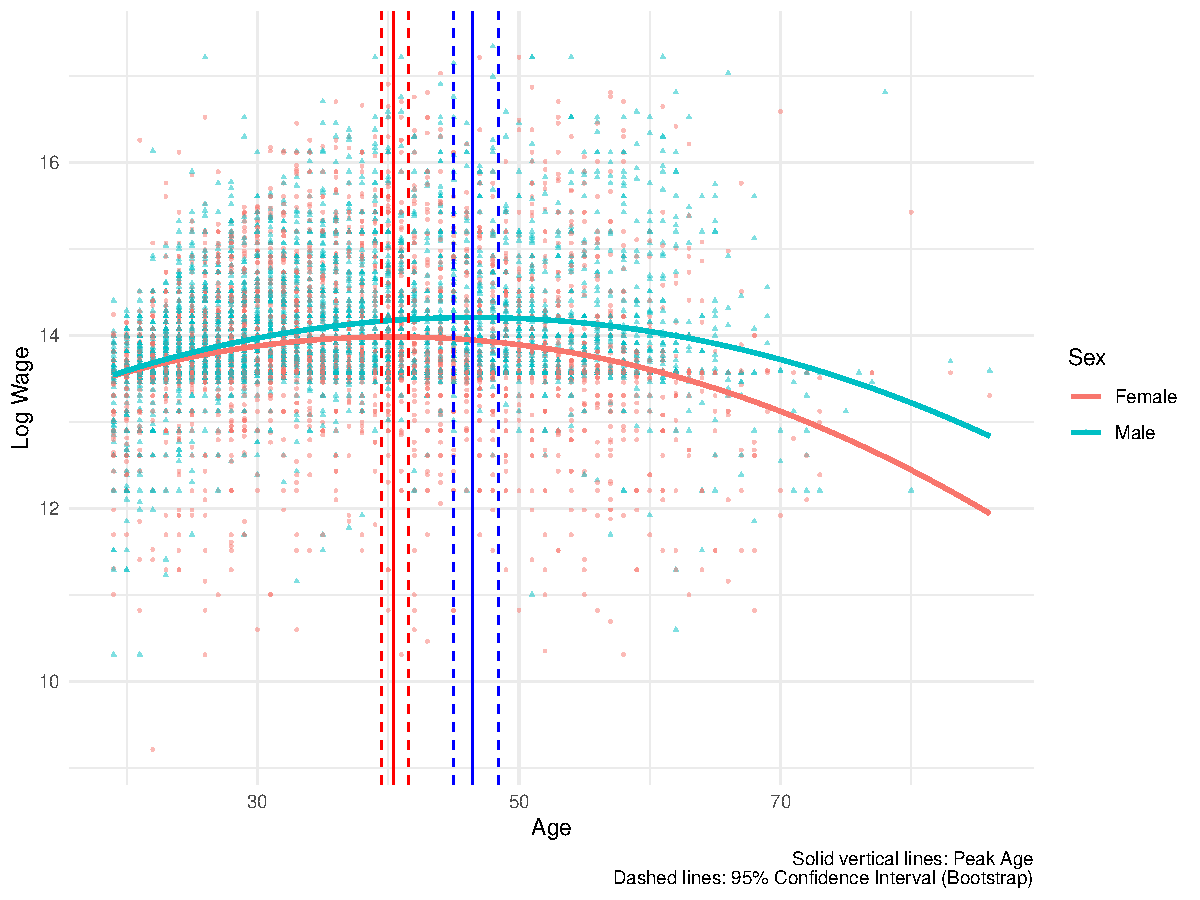
\includegraphics[scale=0.6]{../views/P4_age_logw_sex_profile.pdf}   
            \caption{Age--LogWage Profile by Gender} \label{fig:P4}
        \end{figure}
    
        \begin{figure}[H]
            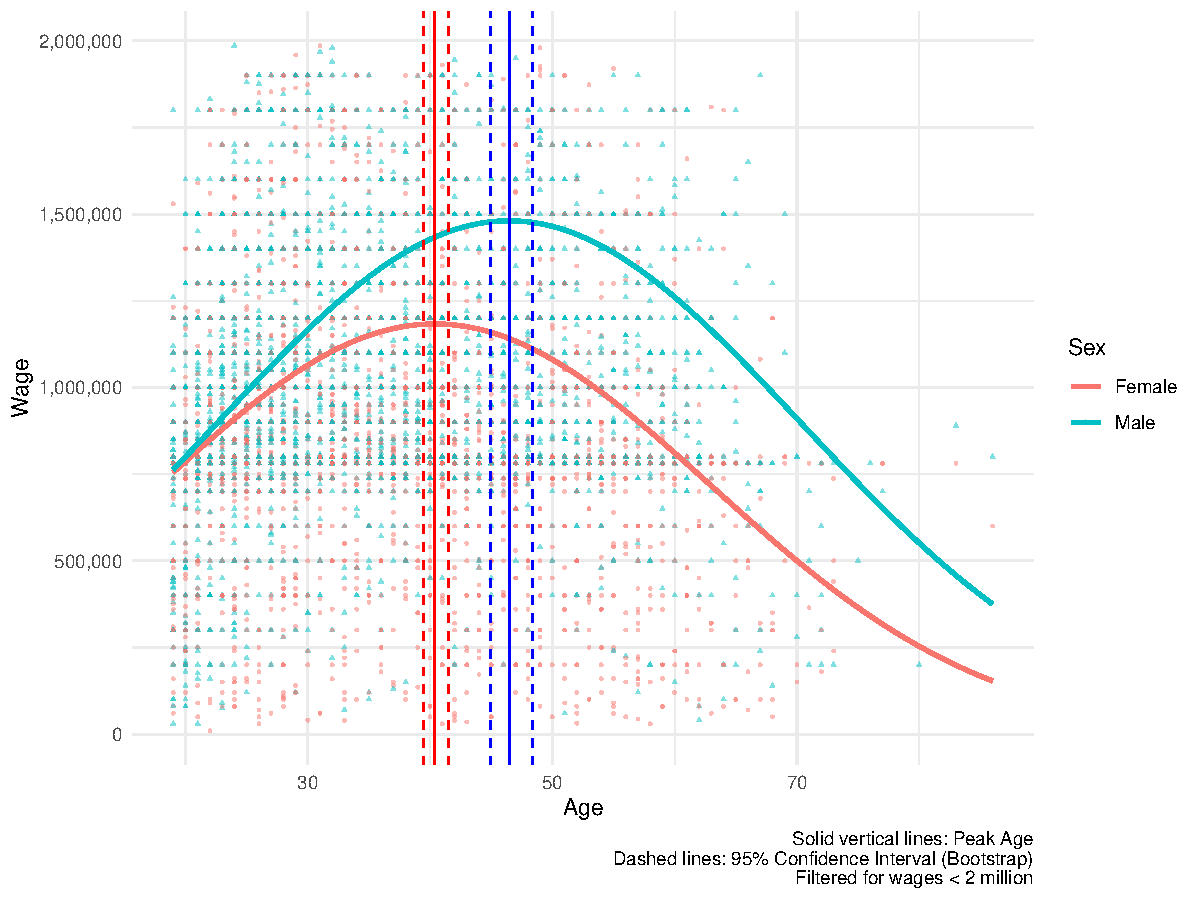
\includegraphics[scale=0.6]{../views/P5_age_wage_sex_profile.pdf}   
            \caption{Age--Wage Profile by Gender} \label{fig:P5}
        \end{figure}
    
        \begin{figure}[H]
            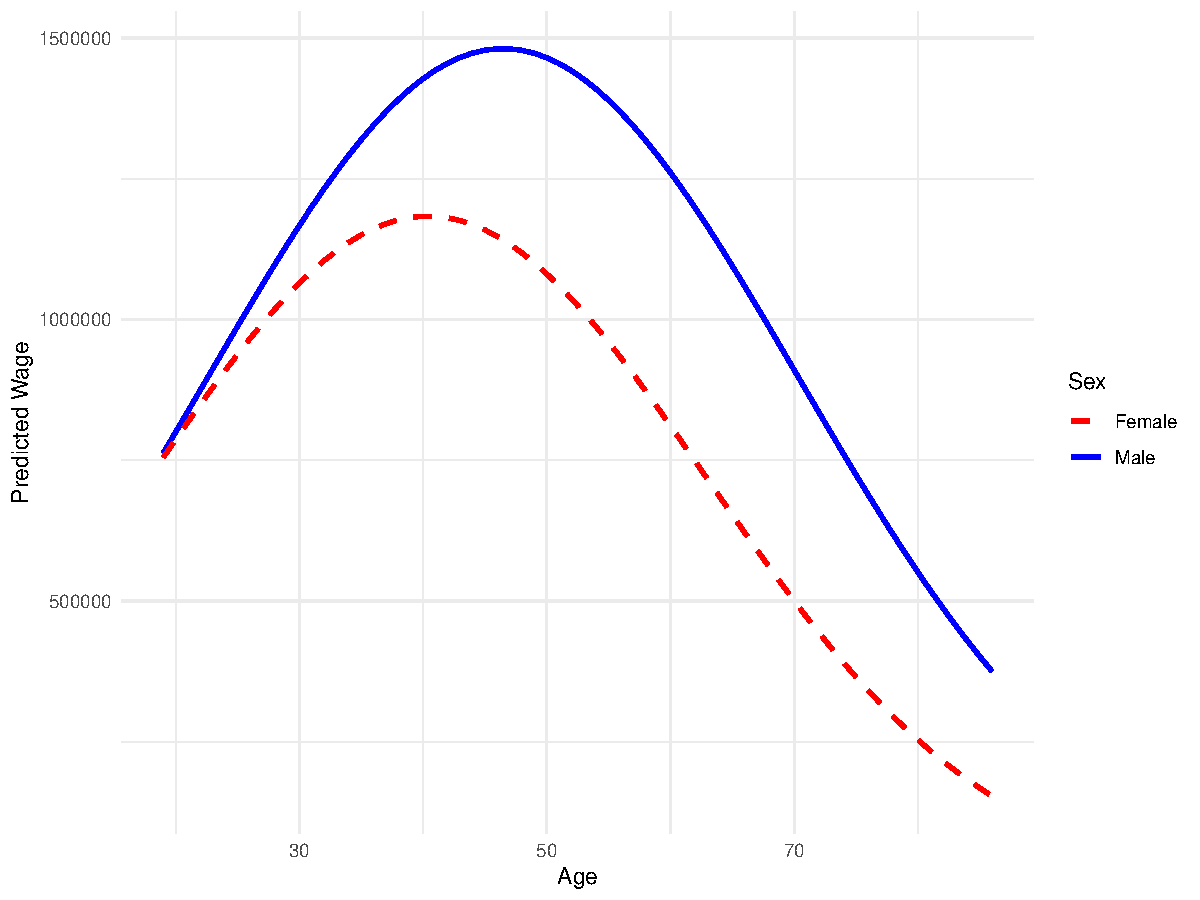
\includegraphics[scale=0.6]{../views/P6_age_wage_sex_profile.pdf}   
            \caption{Predicted Age--Wage  by Gender} \label{fig:P6}
        \end{figure}



% ---------------------------------------------------------------- %
% --------------------- PREDICTING EARNINGS ---------------------- %
% ---------------------------------------------------------------- %
\section{Predicting Earnings}

   \subsection{Training-Test}

        In order to ensure the reproducibility of our results and to train the model effectively, we divided the dataset into a training set (70\%) and a test set (30\%). A seed value was set to guarantee that this split can be replicated. This approach allows us to estimate the model on one portion of the data and then assess its performance on a separate subset, ensuring that the model is not overfitted to the training data and that it generalizes well to unseen observations. The models we will analyze include three key specifications: the quadratic age model, the unconditional gender wage gap model, and the conditional gender wage gap model. These models serve as the foundation for understanding the relationship between age, gender, and wages. In addition to these core models, we estimated five additional models to explore non-linearities and complexities in the age-wage profile and gender wage gap. These five additional models include a variety of specifications, incorporating controls and interactions designed to capture more intricate patterns in the data. vThe models can be specified as follows:
        
        \begin{itemize}
            \item \textbf{Model 4:} This model includes age, age squared, gender, and a broad set of control variables.
            \begin{align*}
            \log(w) &= \beta_1 + \beta_2 Age + \beta_3 Age^2 + \beta_4 Female + \beta_5 HoursWorked + \beta_6 Formality \\
            &+ \beta_7 Relab + \beta_8 Education + \beta_9 Stratum + \beta_{10} FirmSize + u \tag{4}
            \end{align*}
            
            \item \textbf{Model 5:} This specification introduces the logarithm of hours worked and firm size.
            \begin{align*}
            \log(w) &= \beta_1 + \beta_2 Age + \beta_3 Age^2 + \beta_4 Female + \beta_5 \log(HoursWorked) + \beta_6 Formality \\ &+ \beta_7 Relab + \beta_8 Education + \beta_9 Stratum + \beta_{10} \log(FirmSize) + u \tag{5}
            \end{align*}
            
            \item \textbf{Model 6:} This model adds multiple interaction terms to examine how gender interacts with age, hours worked, and other covariates.
            \begin{align*}
            \log(w) &= \beta_1 + \beta_2 Age + \beta_3 Age^2 + \beta_4 Female + \beta_5 HoursWorked + \beta_6 Formality \\
            &+ \beta_7 Relab + \beta_8 Education + \beta_9 Stratum + \beta_{10} FirmSize \\ &+ \beta_{11} (Female \times Age) + \beta_{12} (Female \times HoursWorked) \\ &+ \beta_{13} (Age \times Education) + \beta_{14} (HoursWorked \times Relab) + u \tag{6}
            \end{align*}
            
            \item \textbf{Model 7:} This specification combines logarithmic transformations with interaction terms.
            \begin{align*}
            \log(w) &= \beta_1 + \beta_2 Age + \beta_3 Age^2 + \beta_4 Female + \beta_5 \log(HoursWorked) + \beta_6 Formality \\ &+ \beta_7 Relab + \beta_8 Education + \beta_9 Stratum + \beta_{10} \log(FirmSize) \\
            &+  \beta_{11} (Female \times Age) +  \beta_{12} (Female \times \log(HoursWorked)) \\ &+ \beta_{13} (Age \times Education) +  \beta_{14} (\log(HoursWorked) \times Relab) + u \tag{7}
            \end{align*}
            
            \item \textbf{Model 8:} The final model introduces a more complex specification with polynomial terms for age.
            \begin{align*}
            \log(w) &= \beta_1 + \sum_{m=0}^{3} \beta_2 Age^m + \beta_4 Female + \beta_5 \log(HoursWorked) + \beta_6 Formality \\ &+ \beta_7 Relab + \beta_8 Education + \beta_9 Stratum + \beta_{10} \log(FirmSize) \\ &+ \sum_{m=0}^{3} (\beta_{11} Age^m \times Female) + \sum_{m=0}^{3} (\beta_{12} Age^m \times Education) \\ &+ \sum_{m=0}^{3} (\beta_{13} Age^m \times Relab) + u \tag{8}
            \end{align*}
        \end{itemize}

        
        The control variables included in these models, such as \textit{relab} (employment relationship), \textit{hoursWorkUsual} (hours worked), \textit{formal} (formality of employment), \textit{sizeFirm} (firm size), and \textit{maxEducLevel} (education level), are justified based on their known importance in determining wages. Each variable plays a significant role in influencing the earnings of individuals and helps isolate the impact of gender and age on wage outcomes."


        
\begin{table}[ht]
\centering
\begin{tabular}{lc}
\hline
Model & RMSE \\
\hline
1 &  0.7633  \\
2 &  0.7741  \\
3 &  0.6725  \\
4 &  0.545  \\
5 &  0.5282  \\
6 &  0.54  \\
7 &  0.5248  \\
8 &  0.5236  \\
\hline
\end{tabular}
\caption{RMSE Scores for Different Models}
\label{tab:rmse_scores}
\end{table}
%

        \textit{Table 6} presents the predictive performance of the models estimated in previous sections, evaluated using the Root Mean Square Error (RMSE). RMSE is a widely used metric in regression analysis because it measures the average magnitude of prediction errors, penalizing larger deviations more heavily. This makes it a particularly useful measure for assessing model accuracy. A lower RMSE indicates better predictive performance, as it suggests that, on average, the model’s predictions are closer to the actual observed values. Looking at the results, Model 1 (the unconditional gender wage gap) and Model 2 (the conditional gender wage gap) have the highest RMSE scores, with values of 0.7633 and 0.7741, respectively. This suggests that these simpler models are less effective at predicting wages, likely because they fail to account for the many other factors influencing wages beyond gender. These models only explain a small portion of the variance in wages, as evidenced by the relatively high RMSE values. This aligns with expectations from economic theory, where factors such as education, work experience, industry, and job characteristics play crucial roles in determining wages. The RMSE decreases substantially when moving to Model 3, which includes controls for job characteristics such as hours worked, formality, and firm size. The RMSE drops to 0.6725, indicating a significant improvement in the model's predictive power. This suggests that controlling for these additional variables helps capture more of the underlying determinants of wages, reducing the overall error in predictions.
        
        Models 4 through 8 introduce additional complexity by incorporating non-linearities, interaction terms, and logarithmic transformations. Interestingly, the RMSE continues to decrease as the models become more complex, with Model 8 achieving the lowest RMSE of 0.5236. This result is somewhat counterintuitive, as more complex models often run the risk of overfitting, particularly when they involve numerous interactions and polynomial terms. Overfitting occurs when a model captures noise in the training data, leading to poor generalization to new, unseen data. However, in this case, the more complex models seem to generalize well, at least within the scope of this dataset and the training-testing split. The consistent improvement in RMSE from Models 4 to 8 can be explained by the nature of the problem and the relatively small size of the training set. With only 70\% of the data used for training and 30\% reserved for testing, it is possible that these more complex models do not have enough opportunity to overfit. Additionally, the short duration of the training phase means that the models may not yet be capturing all of the noise in the data, allowing for better generalization to the test set. However, this does not imply that further increases in complexity would continue to improve predictive performance. There is a balance between bias and variance in machine learning, and increasing model complexity can lead to diminishing returns or even worse performance if the model starts to capture too much noise.
        
        Models 5 through 8, in particular, stand out for their relatively low RMSE values, which are all below 0.54. This indicates that incorporating interactions, non-linearities, and logarithmic transformations helps capture more nuanced relationships between age, gender, hours worked, and other job characteristics. For example, the inclusion of interactions between gender and age allows the model to account for the possibility that the effect of age on wages may differ between men and women. Similarly, logarithmic transformations help model diminishing returns to increases in hours worked or firm size, reflecting economic realities where the marginal benefit of additional work hours or firm size may decrease beyond a certain point. In particular, the lowest RMSE is achieved by Model 8, which incorporates polynomial terms for age, interactions between gender and education, and other complex relationships. This suggests that the age-wage relationship is not purely linear or quadratic but may have more intricate patterns that can only be captured by higher-order terms. However, while the RMSE improvements from Models 4 to 8 are encouraging, it is important to note that these gains may not always translate to real-world improvements in understanding or decision-making. Overly complex models can be difficult to interpret and may not provide the same level of insight into the underlying economic relationships.
    
        \begin{figure}[H]
            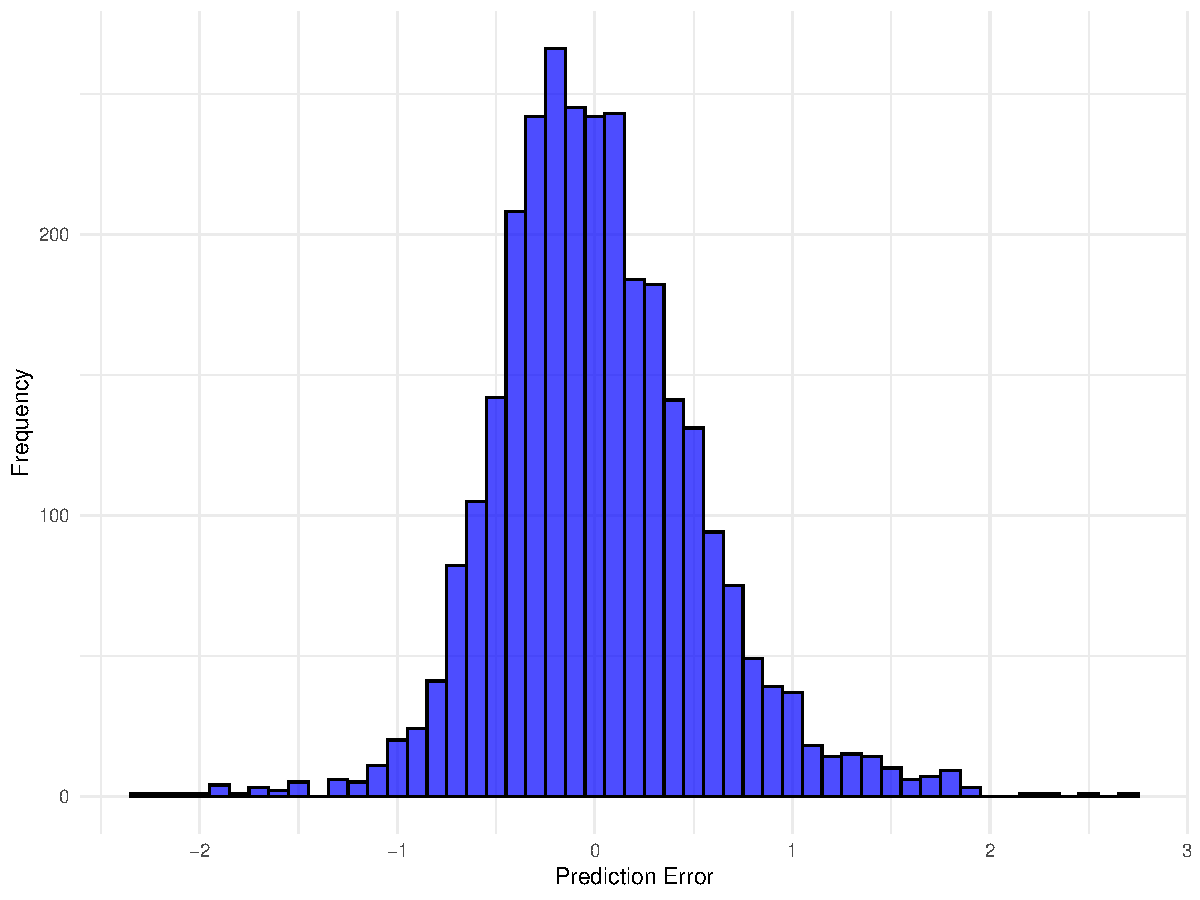
\includegraphics[scale=0.6]{../views/P7_prediction_errors_hist.pdf}   
            \caption{Distribution of Prediction Errors -- Model 8} \label{fig:P7}
        \end{figure}
    
        \begin{figure}[H]
            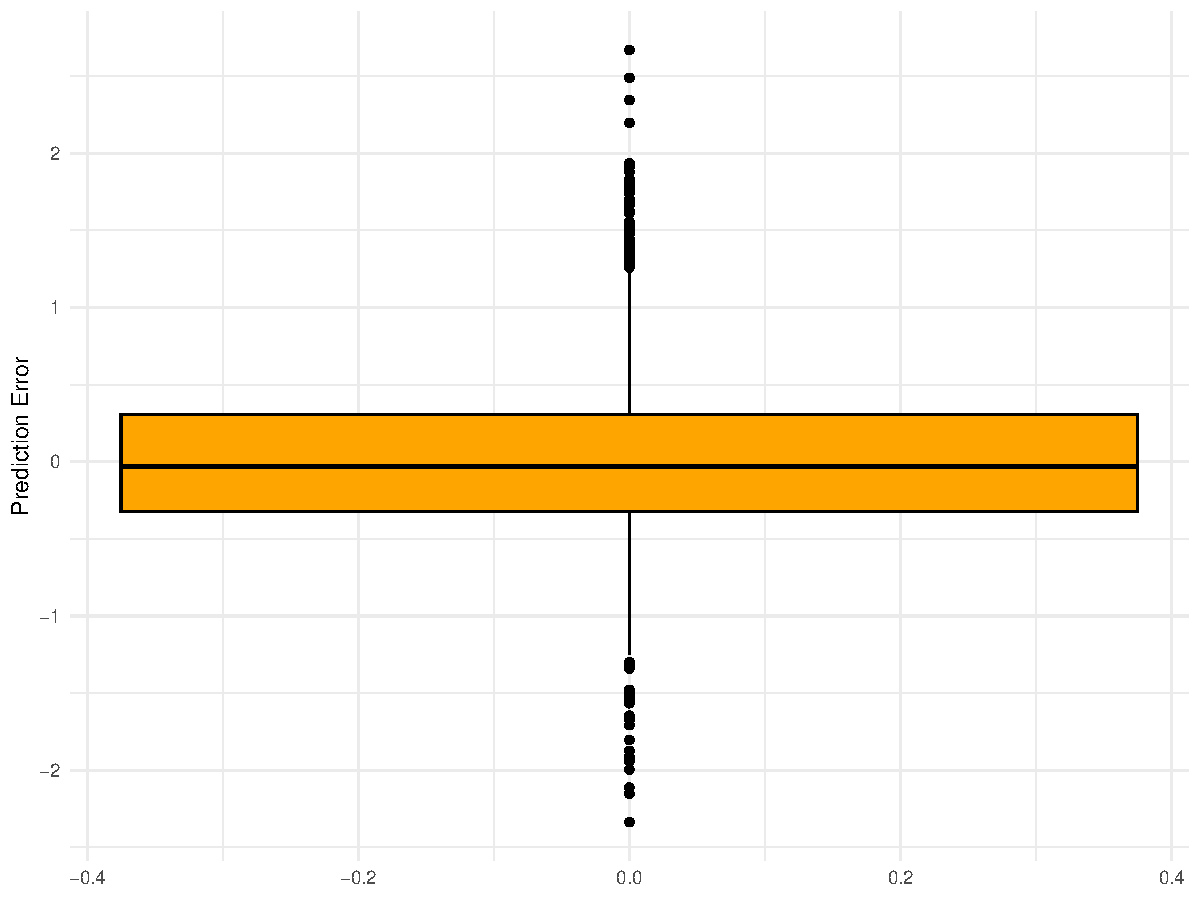
\includegraphics[scale=0.6]{../views/P8_prediction_errors_box.pdf}   
            \caption{Boxplot of Prediction Errors -- Model 8} \label{fig:P8}
        \end{figure}

        The distribution of prediction errors for Model 8 is shown in \textit{Figure 10}, which presents a histogram of the differences between the predicted and actual log wages for the test set. The distribution is approximately normal, with a concentration of errors around zero, suggesting that the model performs well for the majority of observations. However, the tails of the distribution reveal some significant outliers, with prediction errors exceeding 2 on both the positive and negative sides. This indicates that, although the model captures the general trend in wages, there are certain observations where it either significantly overestimates or underestimates wages. These extreme errors warrant further investigation, as they could reflect underlying data issues or important factors that the model has not accounted for.

        \textit{Figure 11} provides further insight into these outliers by showing a boxplot of the prediction errors. The boxplot confirms the presence of a number of extreme outliers, particularly on the lower end, where some individuals have prediction errors below -2. This indicates that the model is drastically overestimating wages for these observations. Conversely, a few individuals have errors greater than 2, suggesting that the model significantly underestimates their wages. While these could be legitimate errors caused by the inherent limitations of the model, it is also possible that these outliers represent individuals who are either underreporting or overreporting their wages. Given that the data comes from the DIAN, an institution responsible for monitoring tax compliance, it is plausible that these extreme outliers could signal individuals who are not accurately reporting their earnings to avoid taxation.
        
        In conclusion, while some of the prediction errors are likely due to model limitations, particularly in capturing the complexity of wage determination across all individuals, the presence of substantial outliers should raise concern. These outliers could be individuals who are underreporting their earnings, either deliberately or due to errors in the data collection process. As a result, the DIAN may want to investigate these cases further to determine whether these extreme prediction errors reflect inaccuracies in wage reporting.

    \subsection{LOOCV}
    
        Leave-one-out cross-validation (LOOCV) is a valuable method in model evaluation because it provides a more reliable estimate of the model’s predictive performance by using every observation in the dataset as both a training and validation point. In contrast to traditional validation set approaches, where a single portion of the data is reserved for testing, LOOCV repeatedly trains the model on all but one observation and tests it on the excluded observation. This process is repeated for every observation in the dataset, and the results are averaged to obtain a final estimate of the model's predictive error. LOOCV is particularly useful in cases where data is limited, as it maximizes the use of available data while minimizing potential bias. However, it is computationally expensive, especially for large datasets, as it requires fitting the model n times, where n is the number of observations.

        The best-performing models identified in the previous analysis, based on their RMSE scores, were Models 5, 7, and 8. These models capture various complexities and non-linearities in the data, with Model 7 exhibiting the lowest RMSE on the test set, followed closely by Model 8. Given that LOOCV provides a more rigorous assessment of model performance, it allows us to evaluate whether these models are truly the best or whether they overfit the training data. The LOOCV results for these models are presented in \textit{Table 7}, alongside the RMSE scores from the traditional test set validation approach.
        
        
\begin{table}[ht]
\centering
\begin{tabular}{lcc}
\hline
Model & RMSE (Test) & RMSE (LOOCV) \\
\hline
5 &  0.5185  &  0.5188  \\
7 &  0.5174  &  0.5168  \\
8 &  0.5159  &  0.5152  \\
\hline
\end{tabular}
\caption{Comparison of RMSE for Models 5, 7, and 8 (Test vs. LOOCV)}
\label{tab:rmse_loocv}
\end{table}
%
        
        The results reveal several important insights into the models' predictive performance. First, there is a remarkable consistency between the RMSE scores obtained through the test set validation and LOOCV for all three models, indicating that the models generalize well across different subsets of the data. However, Model 7 achieves the lowest RMSE score in both the test set and LOOCV, which suggests that it strikes an optimal balance between model complexity and generalization. This outcome reflects the tradeoff between bias and variance, a fundamental concept in machine learning. While more complex models, such as Model 8, are able to capture more intricate patterns in the data (as evidenced by their lower RMSE in the test set), they also introduce higher variance, which can lead to overfitting. In contrast, Model 7 is slightly less complex, which may explain why it performs better under LOOCV, a more rigorous evaluation method that penalize overfitting.
        
        The difference in RMSE between the test set and LOOCV for Model 7 is particularly informative. The fact that Model 7's RMSE improves slightly under LOOCV suggests that it is not overfitting the data and may even benefit from the additional training that LOOCV provides. In contrast, the minimal difference in RMSE for Model 8 indicates that while it performs well on the test set, its additional complexity does not translate into significant performance gains under LOOCV. This underscores the importance of considering both model complexity and generalization when selecting predictive models.
        
        A key link between LOOCV and the influence statistic lies in the sensitivity of the model to individual data points. The influence statistic measures the impact of each observation on the model's coefficients and predictions. LOOCV, by leaving out one observation at a time, inherently captures the influence of each point. If a model has high variance, meaning that it is highly sensitive to small changes in the data, LOOCV will expose this by yielding larger fluctuations in the RMSE when influential data points are omitted. This makes LOOCV a powerful tool for detecting overfitting and identifying influential observations that could disproportionately affect the model’s performance. In our case, the stability of RMSE across both test set validation and LOOCV suggests that none of the models are overly sensitive to any particular observation, further confirming their robustness.
    
    




%%%%%%%%%%%%%%%%%%%%%%%%%%%%%%%%%%%
%		  References				  %
%%%%%%%%%%%%%%%%%%%%%%%%%%%%%%%%%%%

\pagebreak
\singlespacing
\bibliography{References.bib}
Gomez-Cravioto, D.A. et al. (2022). Supervised machine learning predictive analytics for alumni income. J Big Data 9, 11.
\pagebreak


\end{document}

